\documentclass{beamer}

\usecolortheme[light]{solarized}

\beamertemplatenavigationsymbolsempty
\setbeamertemplate{frametitle}[default][center]

\usepackage{hyperref}
\usepackage{minted}

\usepackage{graphicx}
\usepackage{tikz}

\usetikzlibrary{calc, patterns}

\begin{document}

    \begin{frame}
        \begin{center}
            \Large

            Using Python to train my dog.

            \normalsize
            \vspace{1cm}
            \href{https://twitter.com/drvinceknight}{@drvinceknight}\\
            \url{vknight.org}\\
            \texttt{knightva@cardiff.ac.uk}
        \end{center}


    \end{frame}

    \begin{frame}
        \centering

        
\includegraphics[height=2cm]{static/CUident_CMYK.eps}
        \hfill
        
\includegraphics[height=2cm]{static/pyconuk.jpg}
        \hfill
        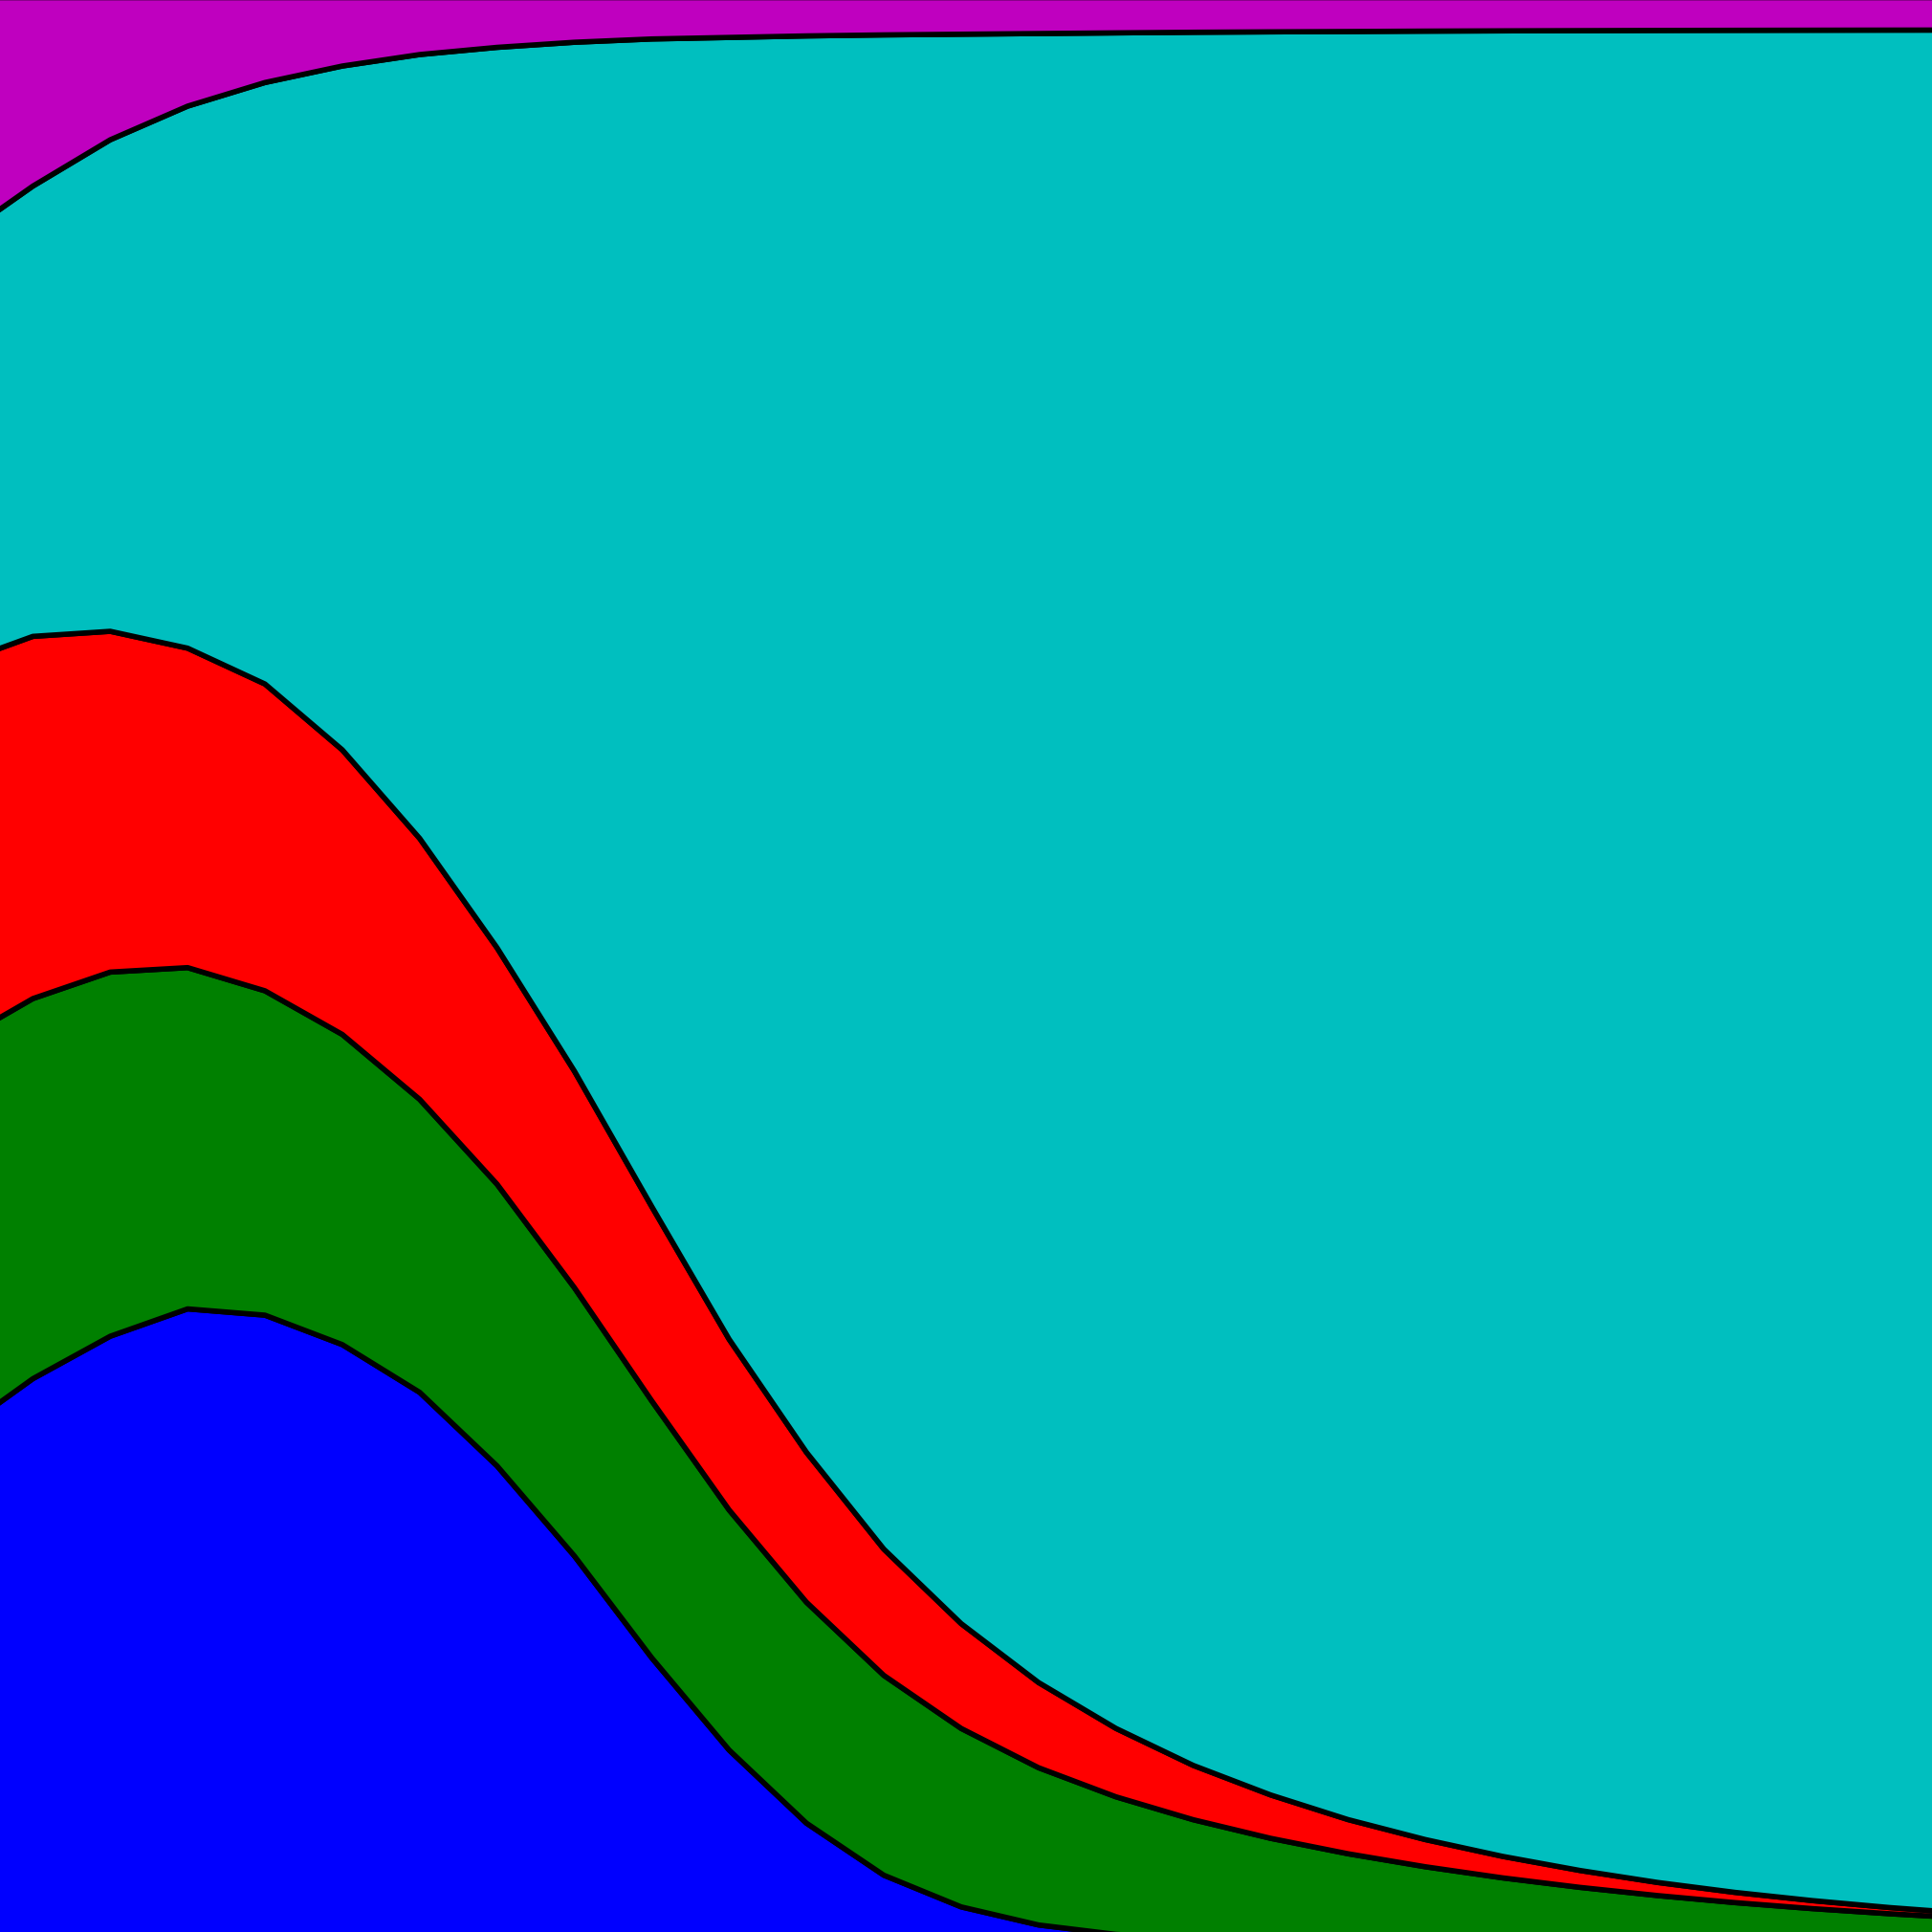
\includegraphics[height=2cm]{static/axelrod_logo.png}
        \hfill
        
\includegraphics[height=2cm]{static/ssi-logo.png}
    \end{frame}

    \begin{frame}
        \centering
        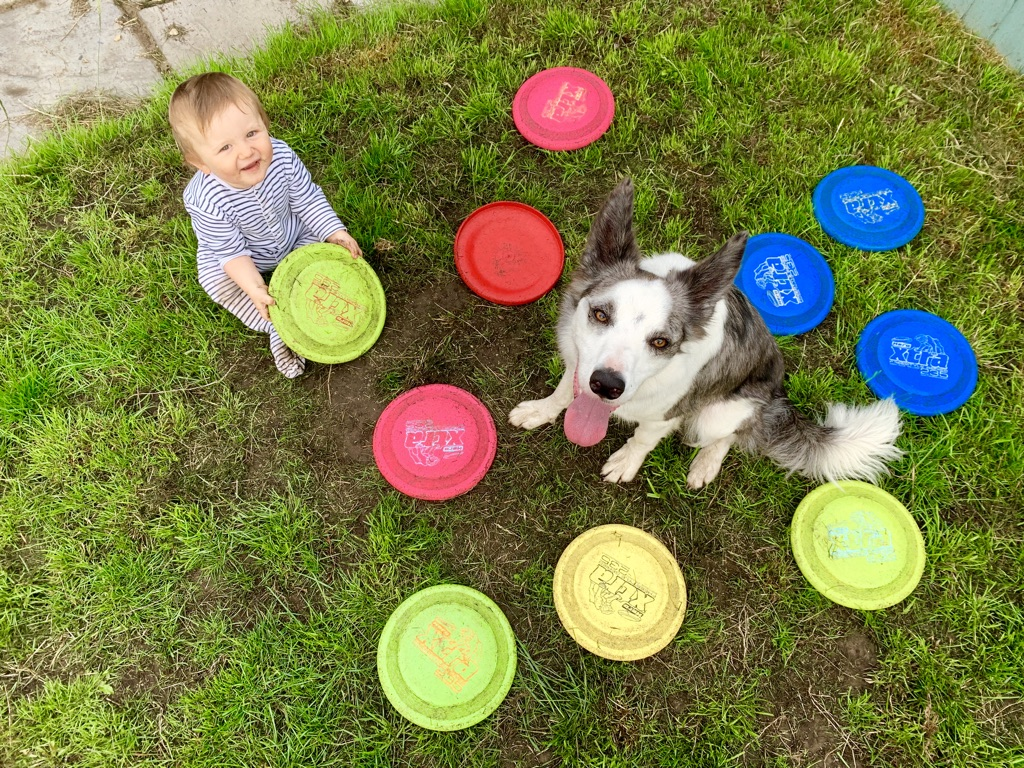
\includegraphics[width=.95\textwidth]{static/jj_and_riggs.jpg}
    \end{frame}

    \begin{frame}
        \centering
        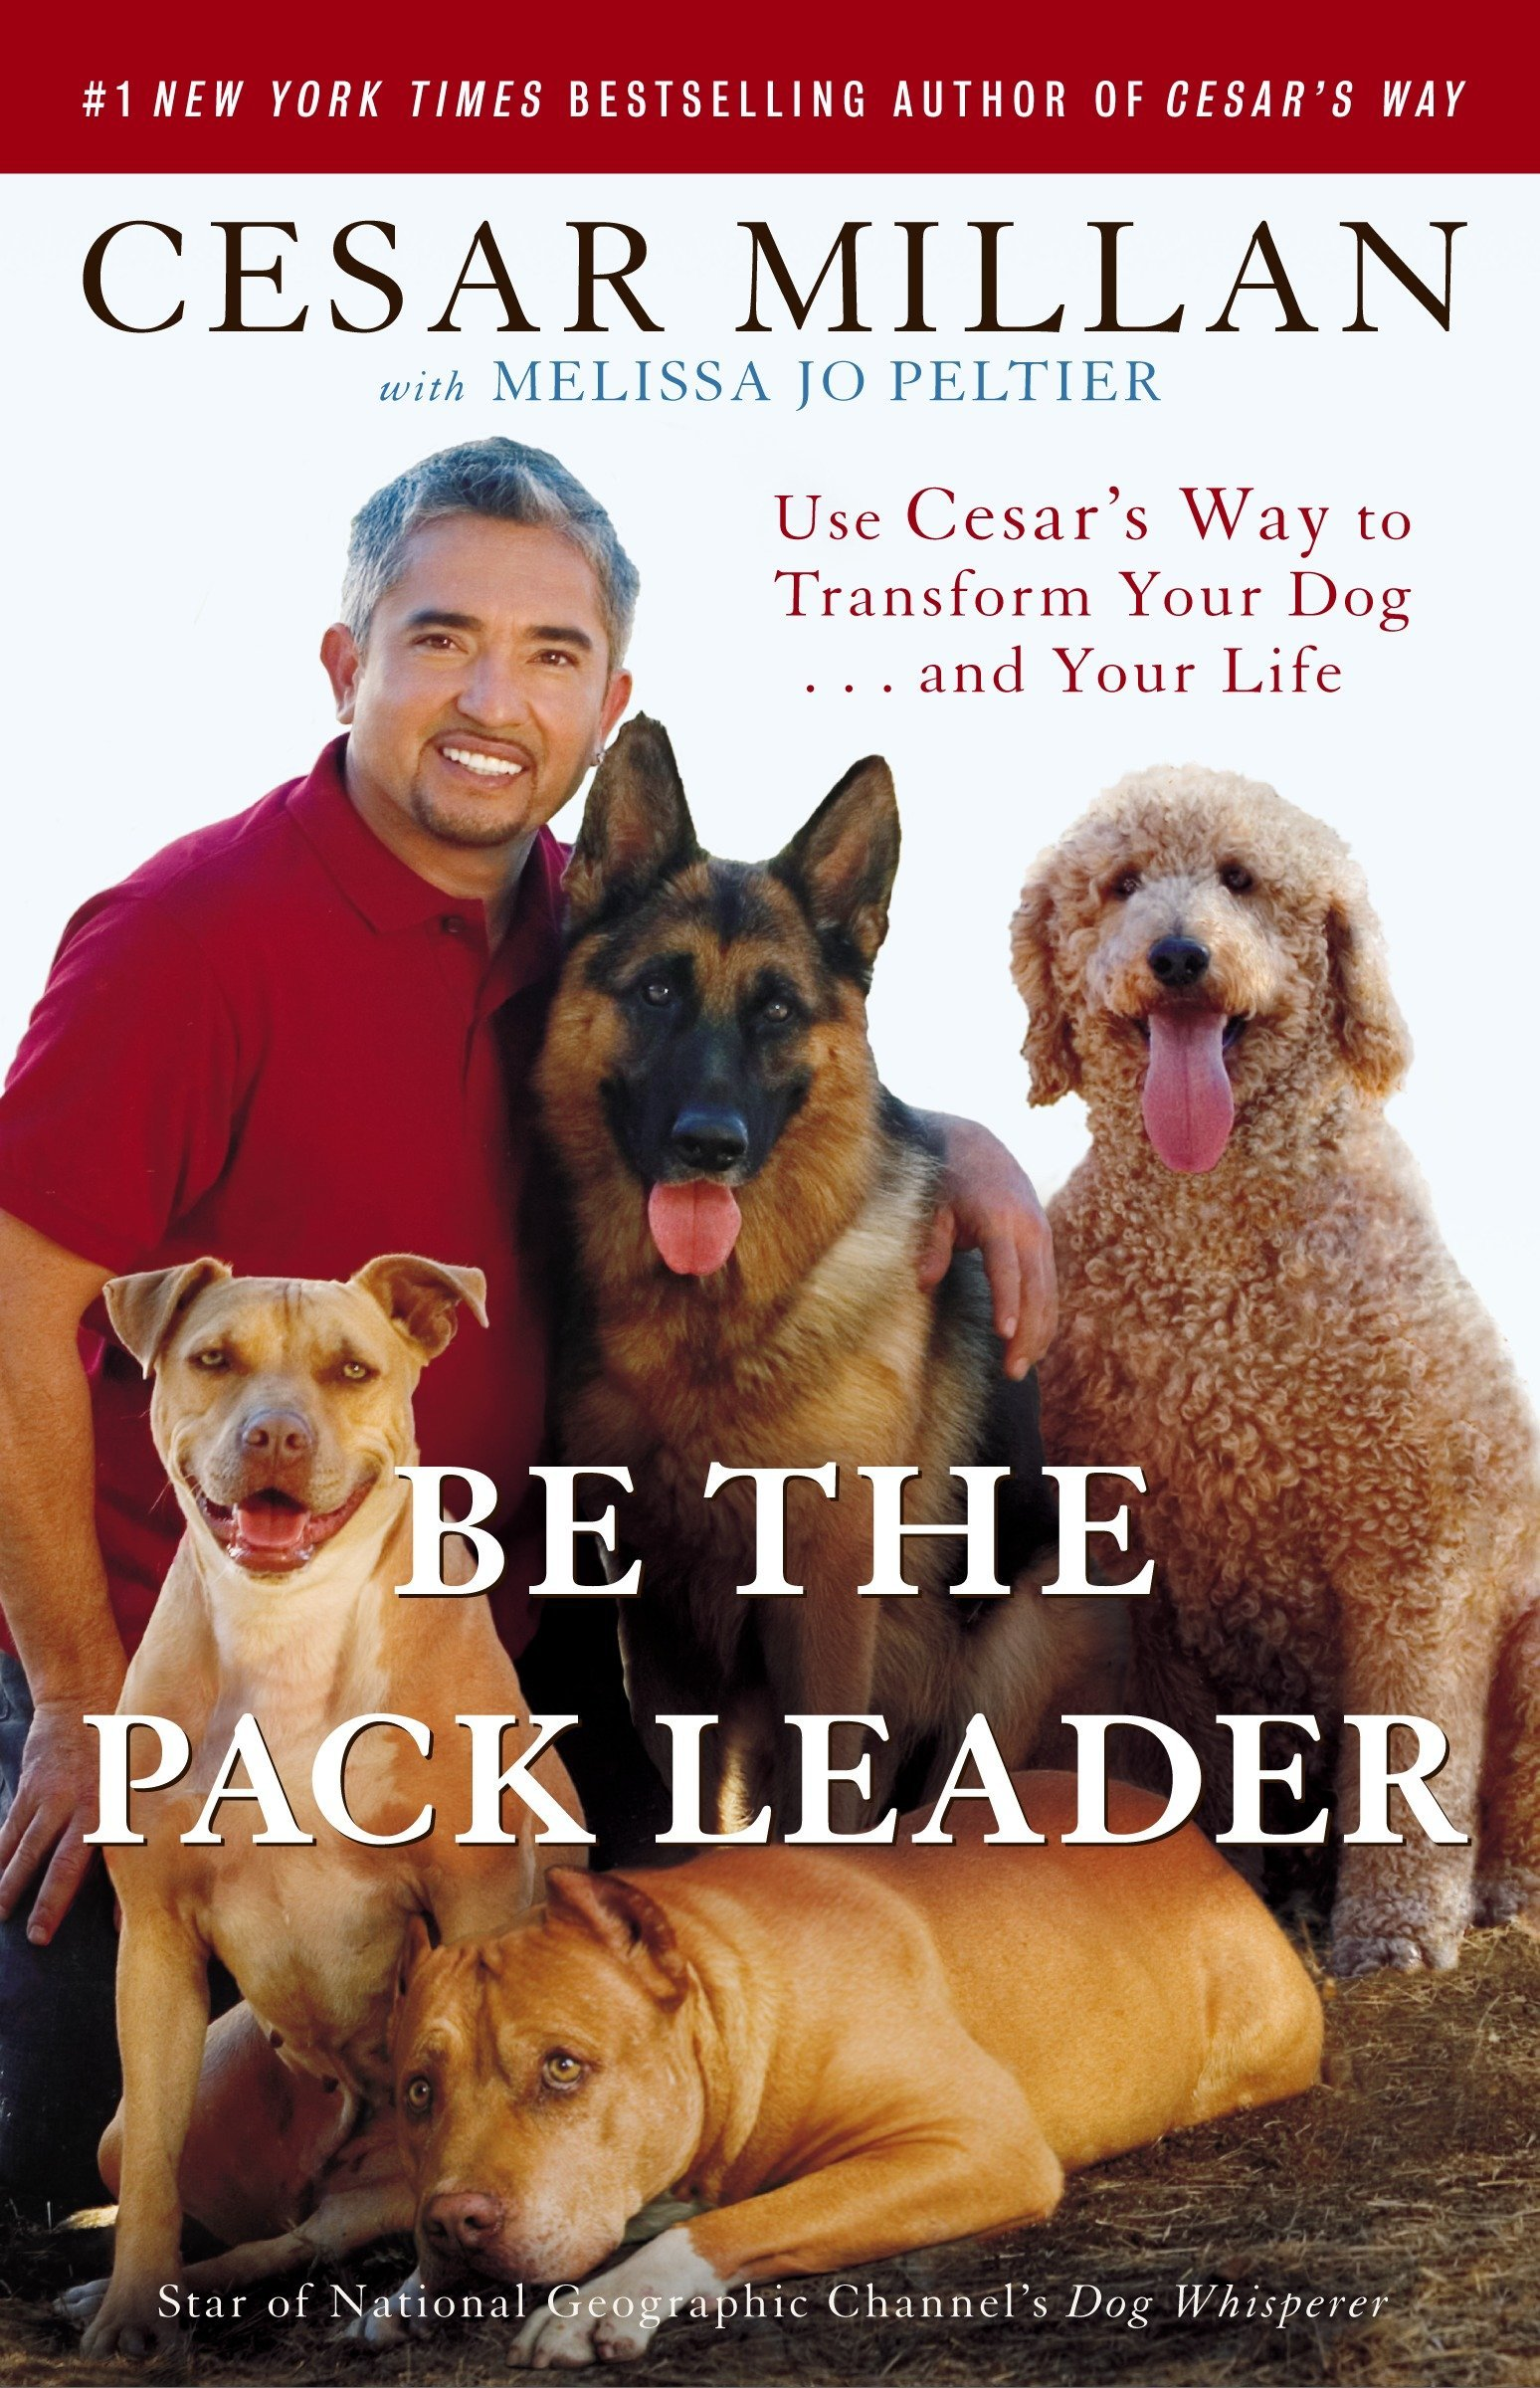
\includegraphics[height=.95\textheight]{static/cesar.jpg}
    \end{frame}

    \begin{frame}
        \centering
        \Huge
        Expression Studies on Wolves - Rudolph Schenkel, 1947
    \end{frame}

    \begin{frame}
        \centering
        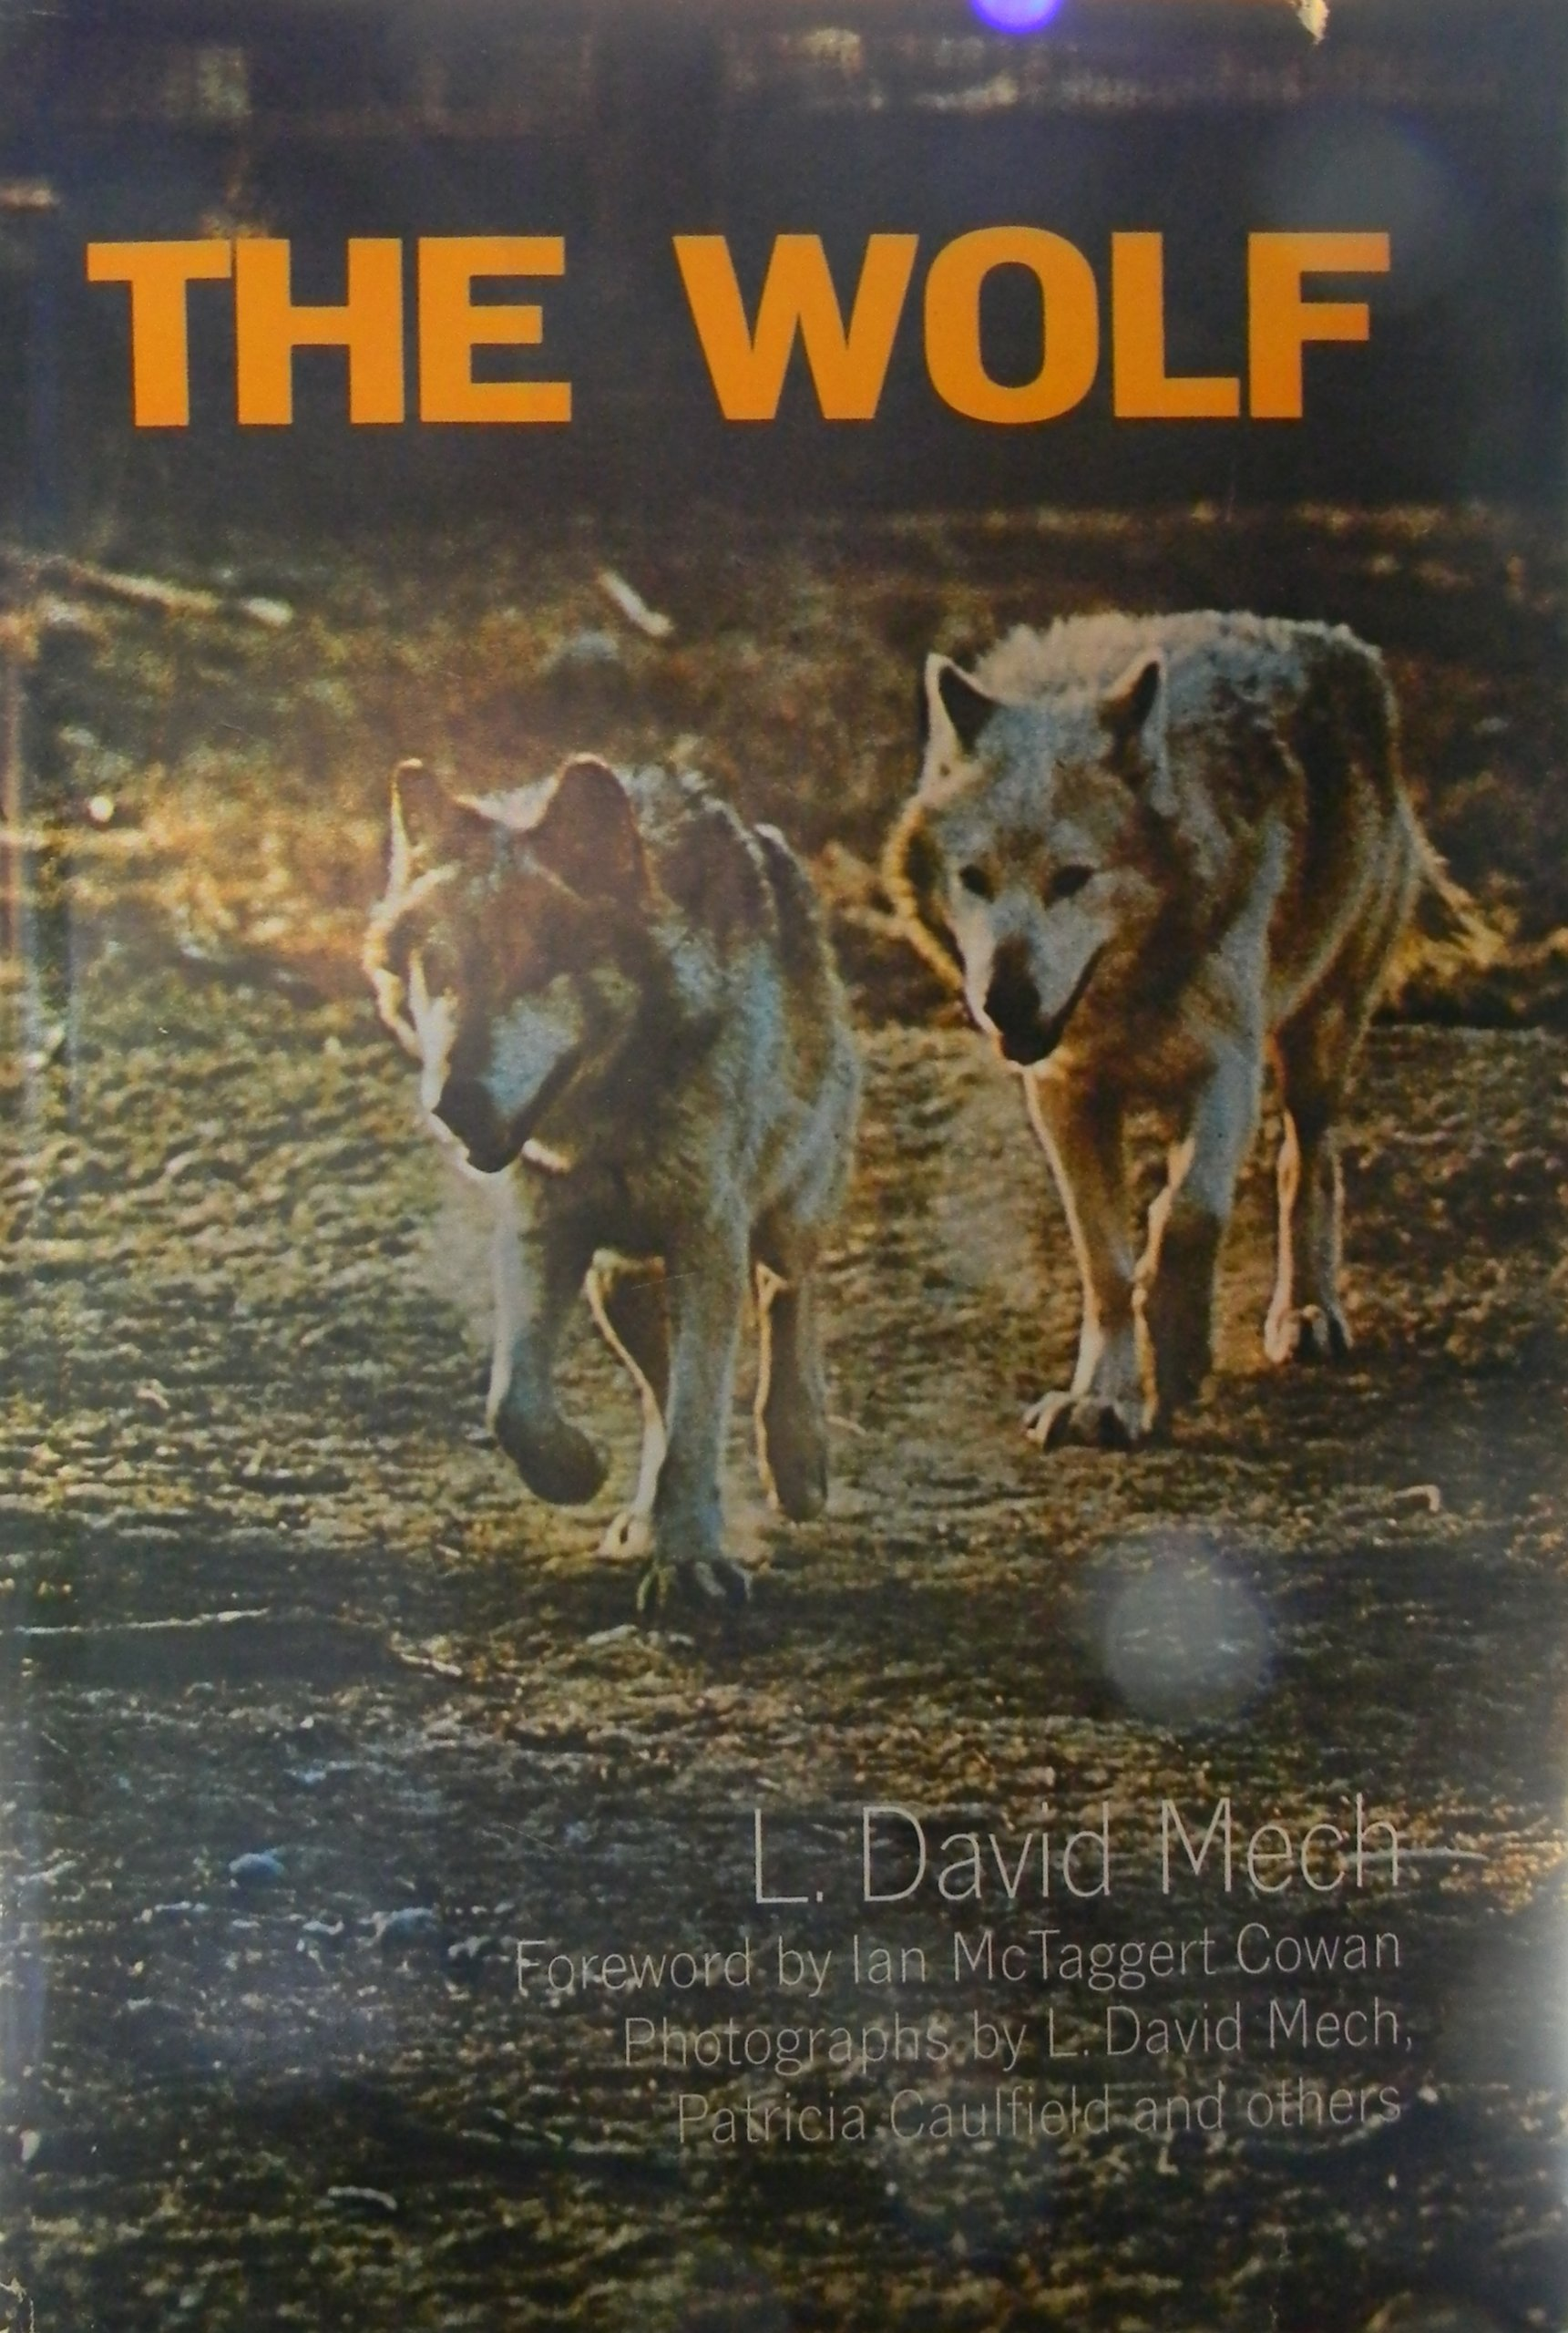
\includegraphics[height=.95\textheight]{static/mech_the_wolf.jpg}
    \end{frame}

    \begin{frame}
        \centering
        \Large
Survey of the use and outcome of confrontational and non-confrontational
training methods in client-owned dogs showing undesired behaviors - Herron et al.
2009
    \end{frame}

    \begin{frame}
        \centering
        \huge
    Alpha Status, Dominance, and Division of Labor in Wolf Pack - David Mech
    2013
    \end{frame}

    \begin{frame}
        \centering
        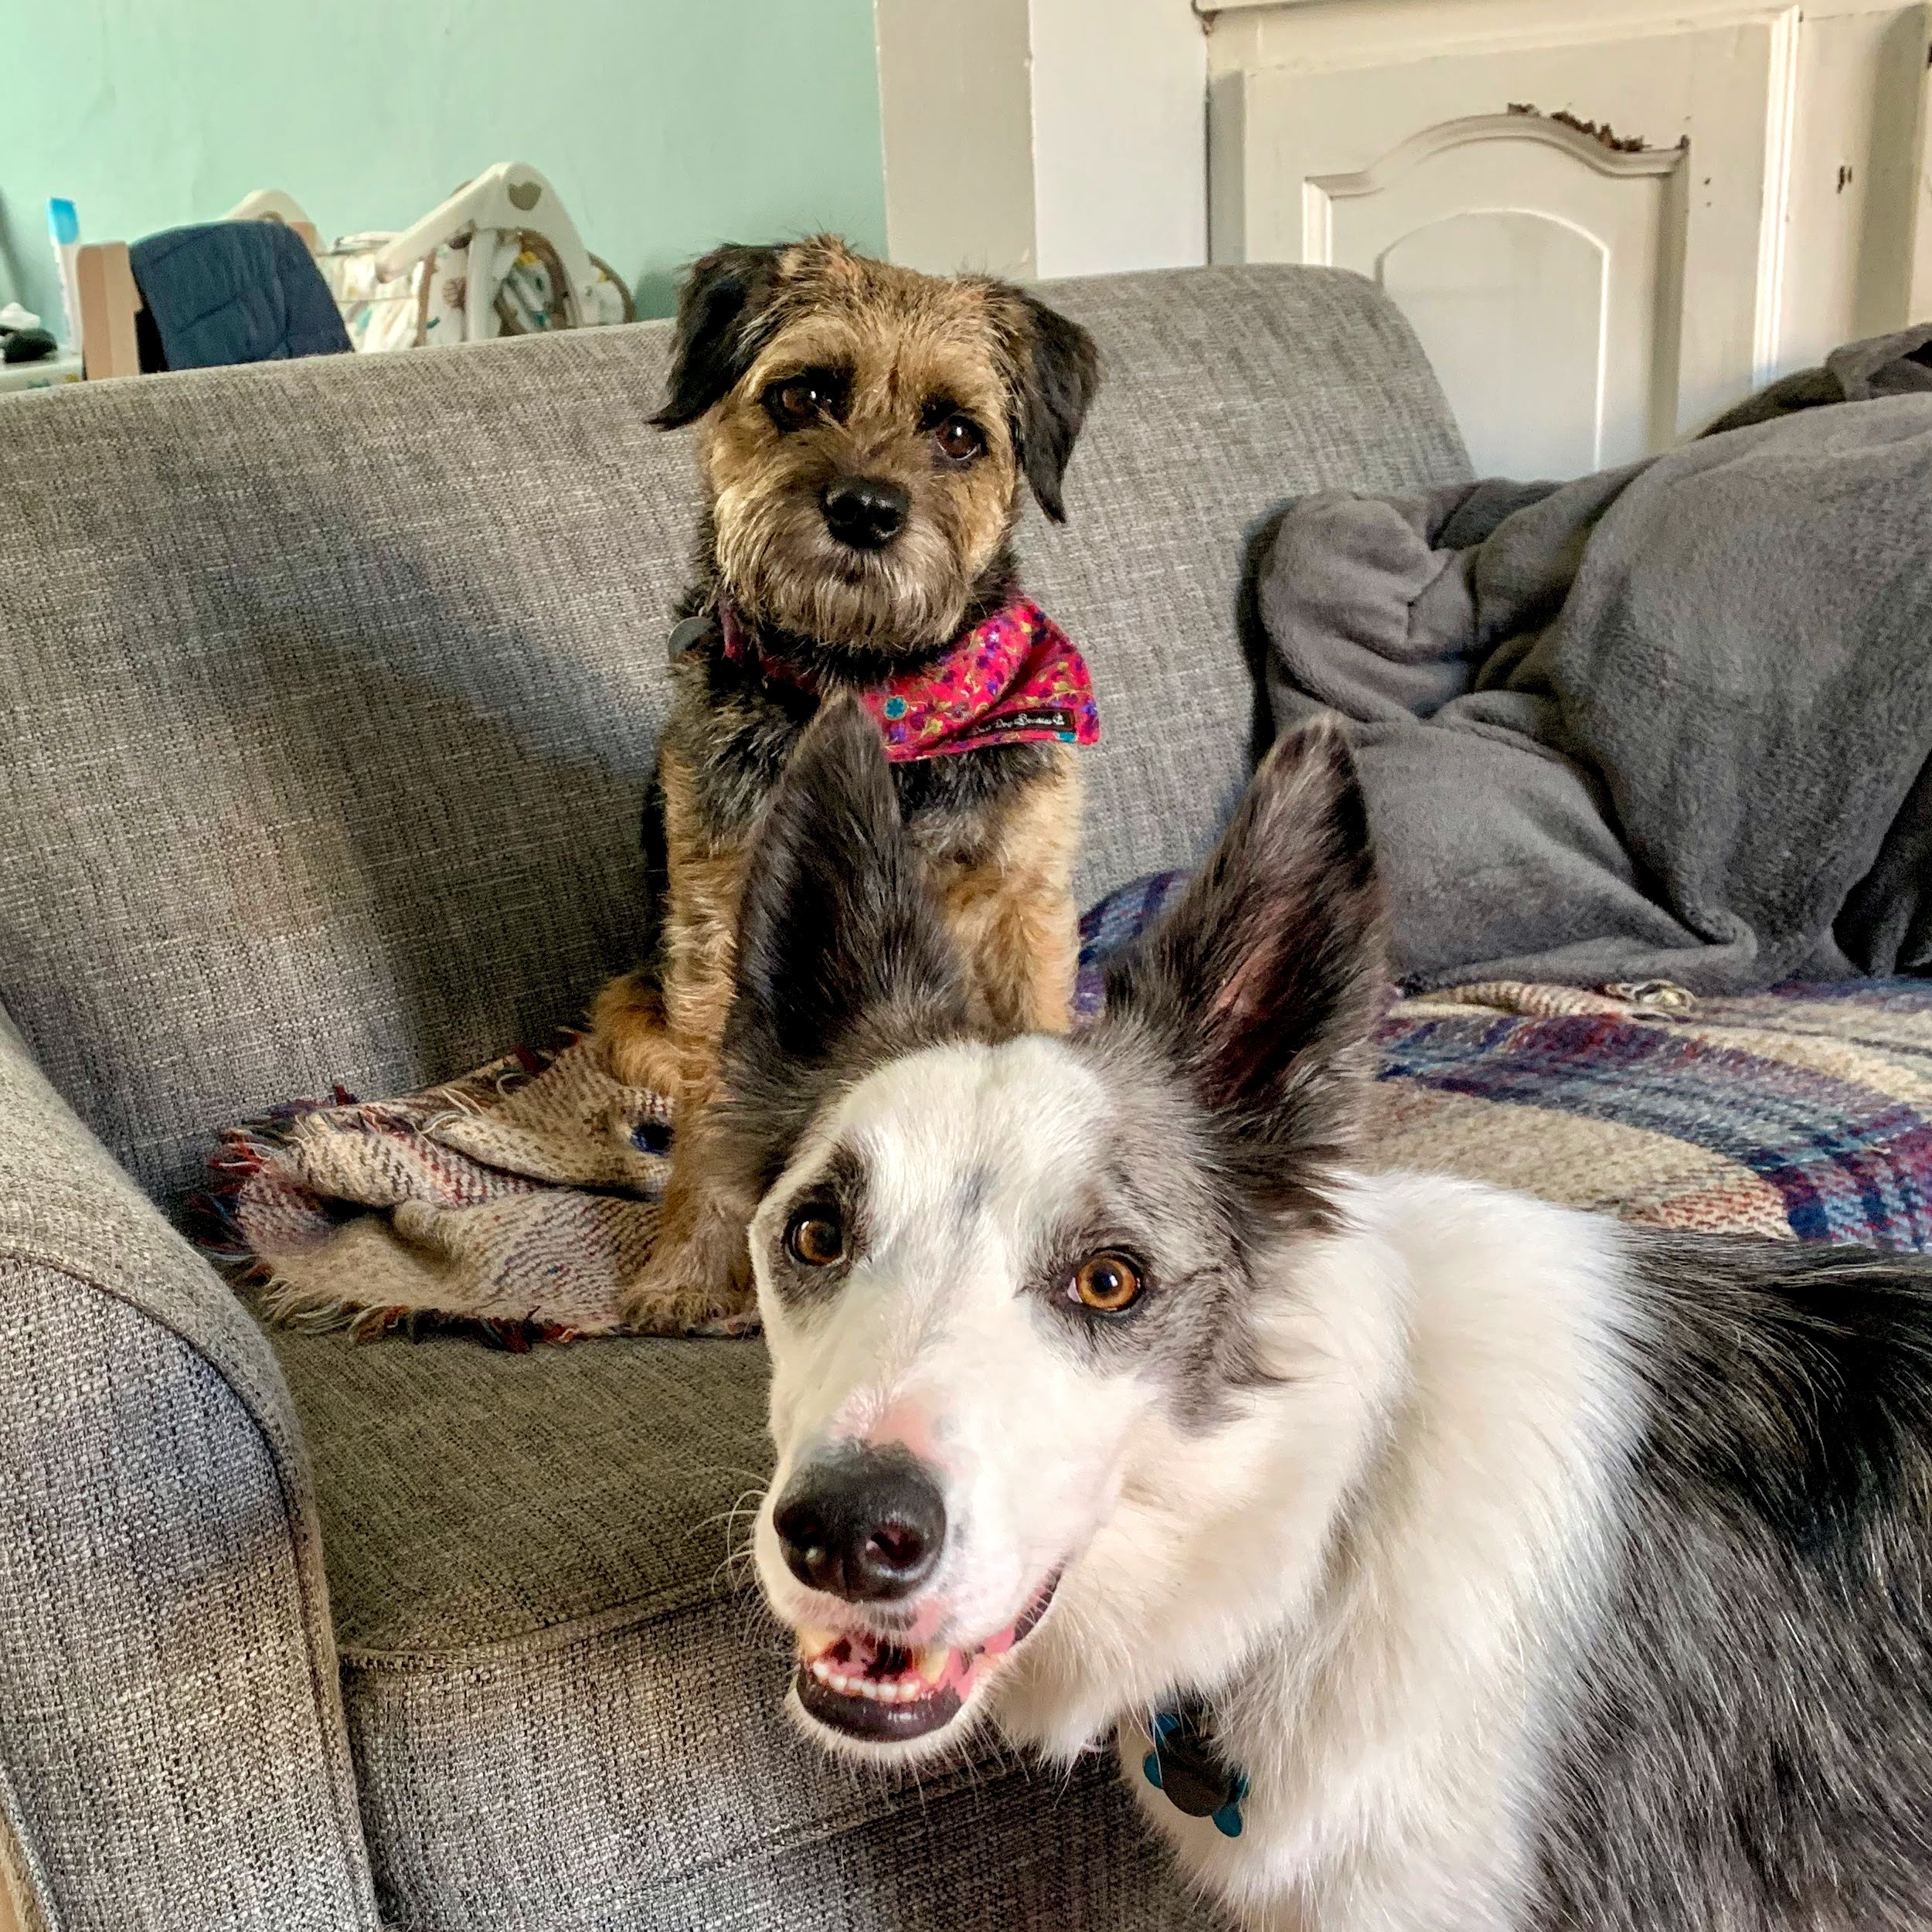
\includegraphics[height=.95\textheight]{static/tobi_and_riggs.jpg}
    \end{frame}


    \begin{frame}
        \centering 
        \LARGE
        
        Behaviouralism \(\to\) Social constructivism

        \vspace{1cm}
        \large
        \url{https://vknight.org/tch-phi/}
    \end{frame}

    \begin{frame}
        \centering
        \Huge
        1. Health
    \end{frame}

    \begin{frame}
        \centering
        \Huge
        2. Companionship
    \end{frame}

    \begin{frame}
        \centering
        \Huge
        3. Diet
    \end{frame}

    \begin{frame}
        \centering
        \Huge
        4. Environment
    \end{frame}

    \begin{frame}
        \centering
        \Huge
        5. Behaviour
    \end{frame}

    \begin{frame}
        \centering
        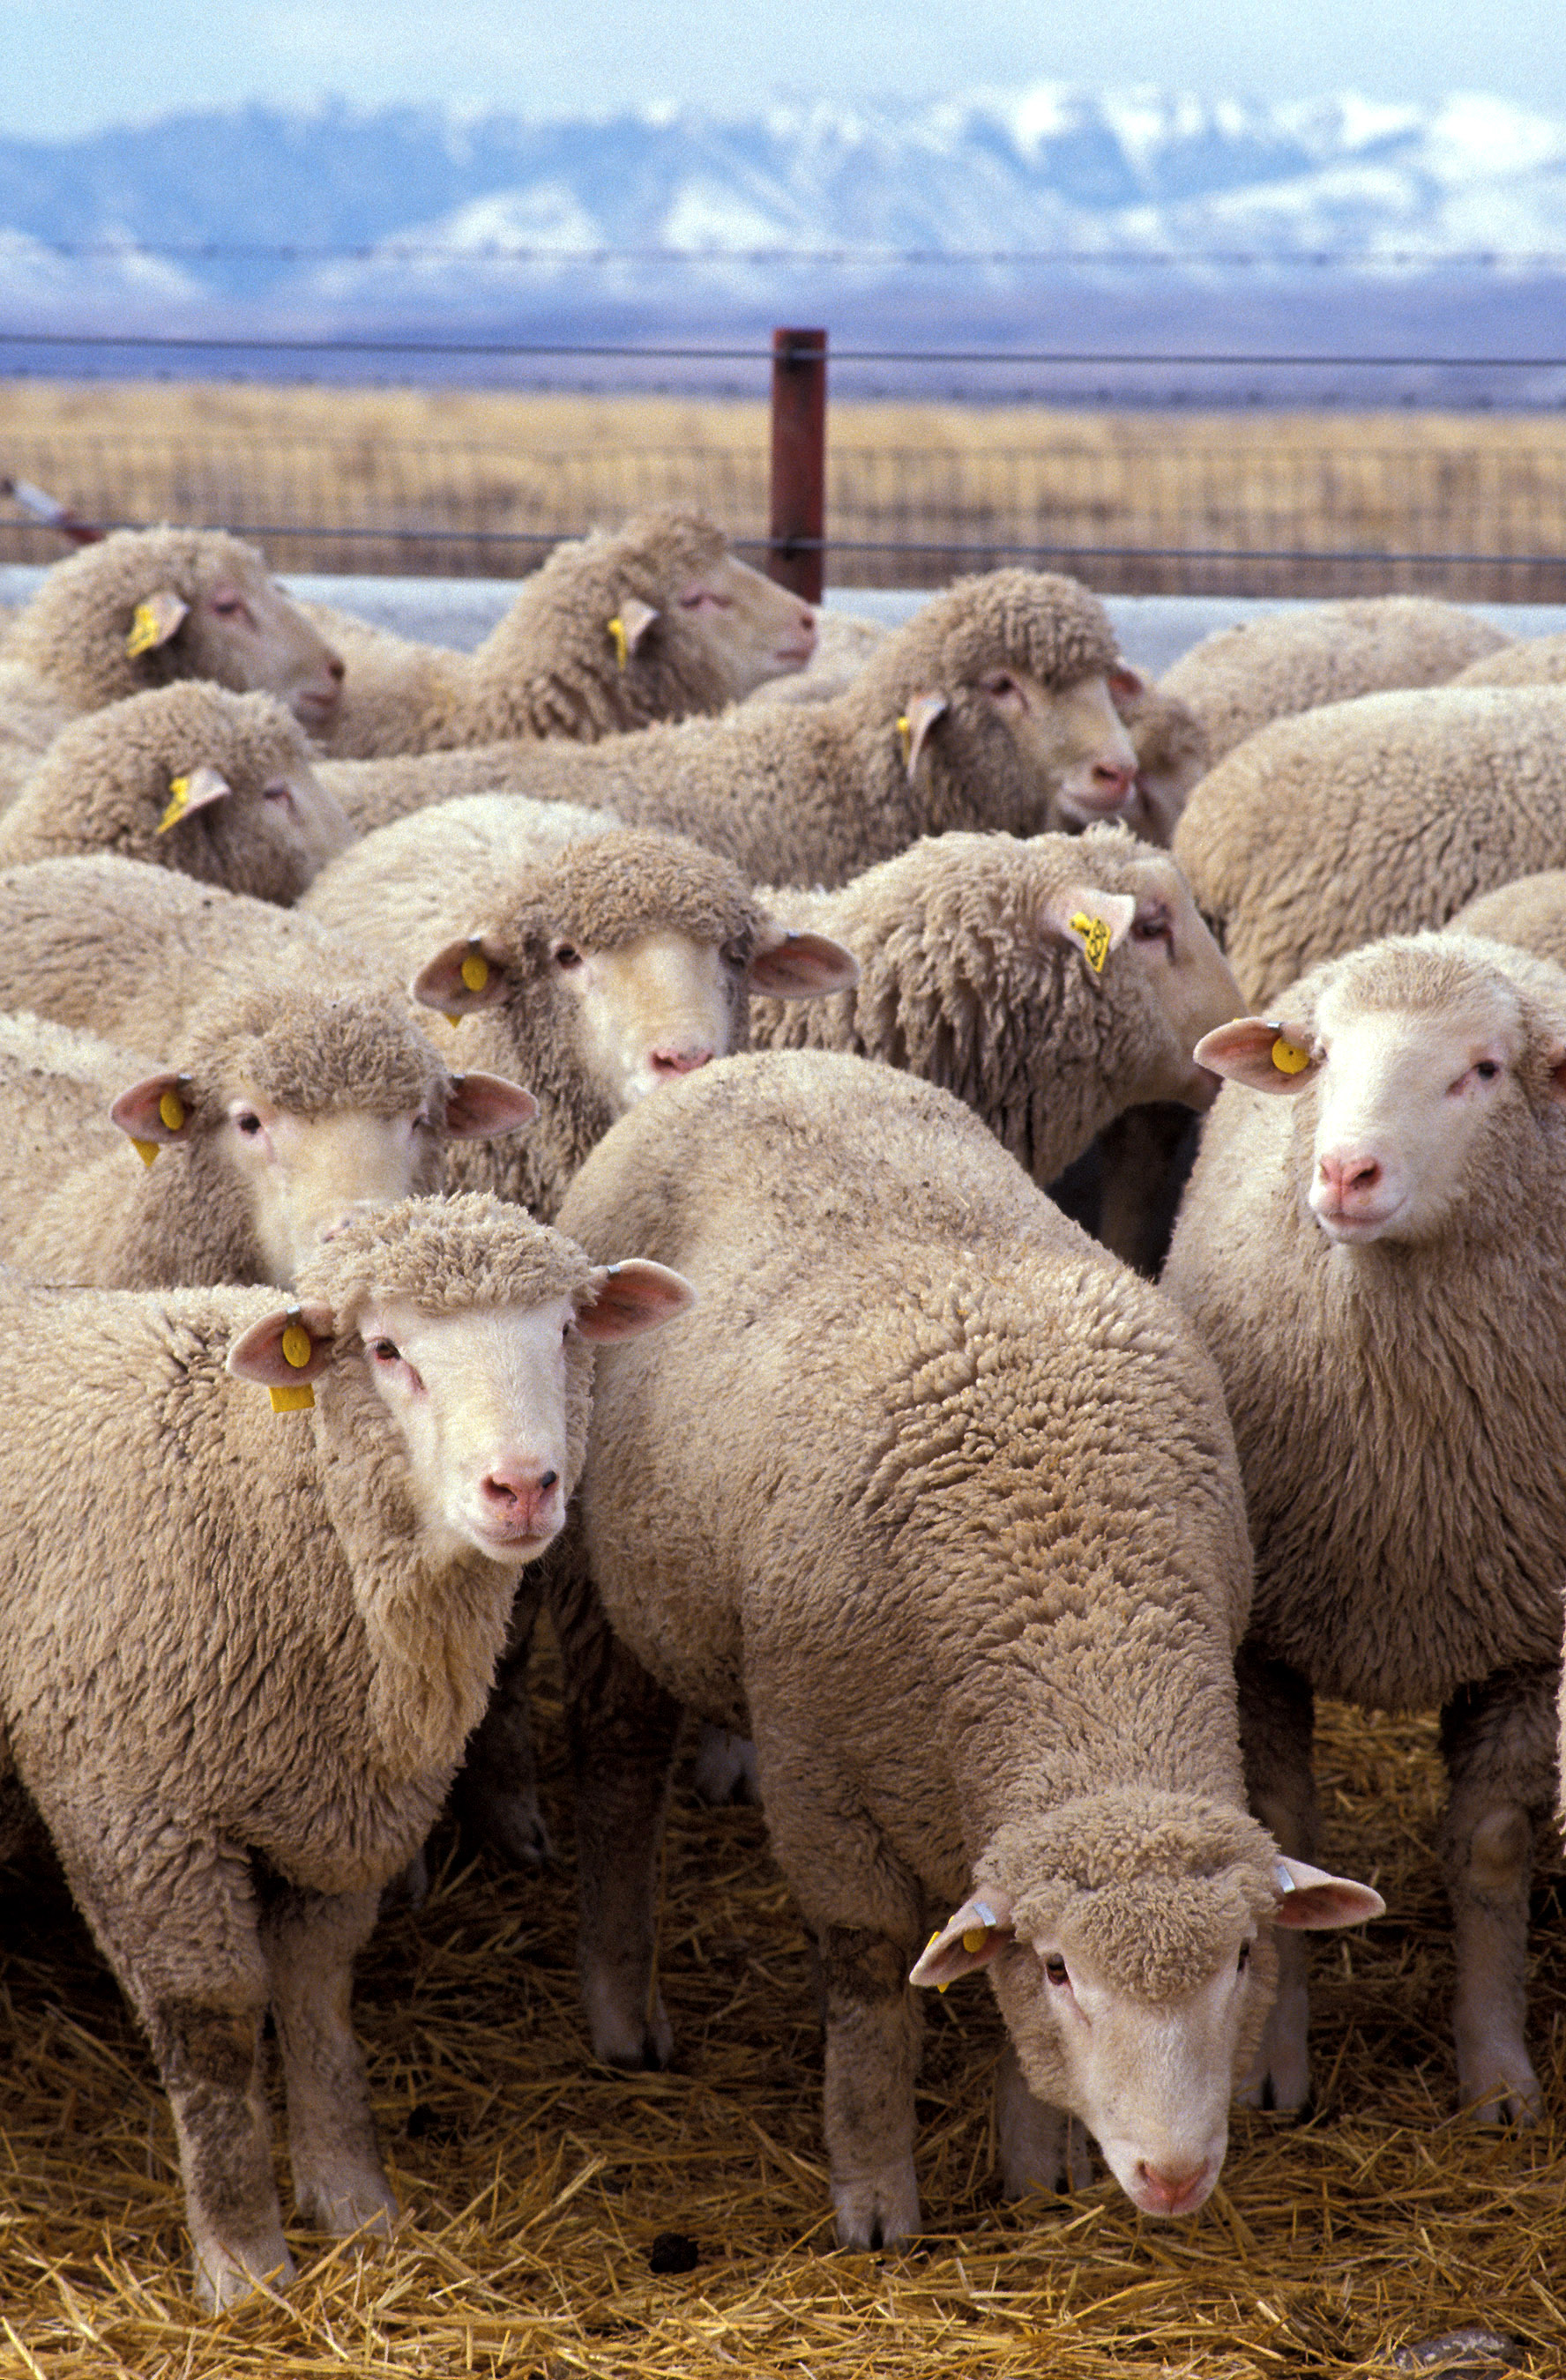
\includegraphics[height=.95\textheight]{static/flock_of_sheep.jpg}
    \end{frame}

    \begin{frame}
        \centering
        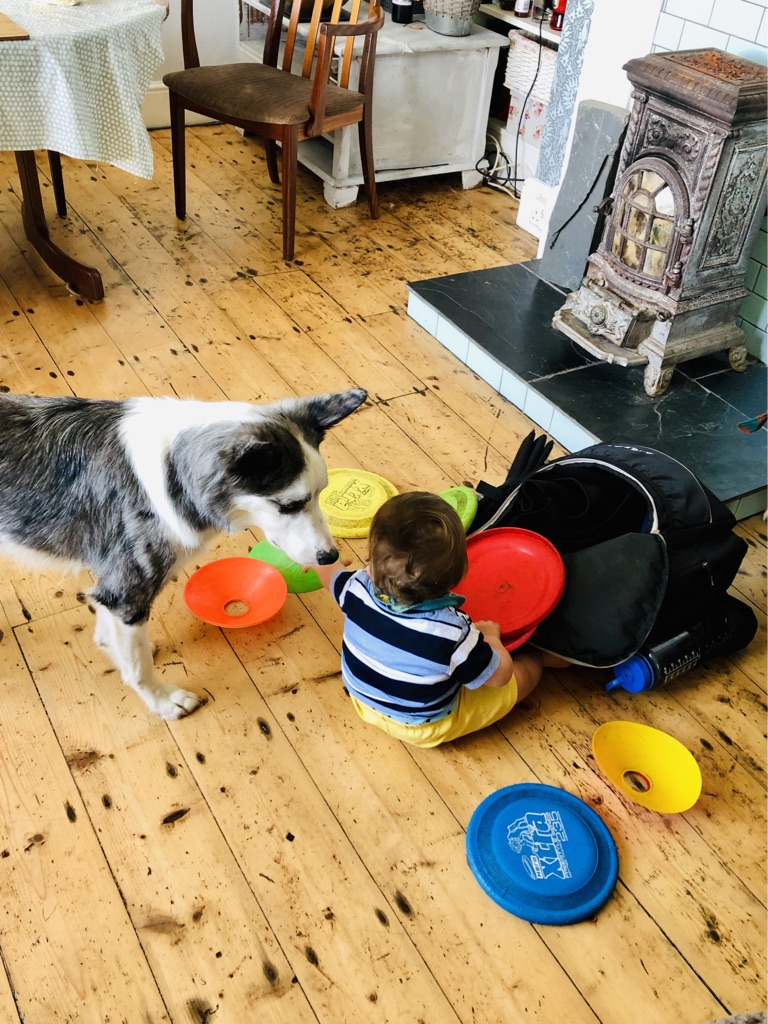
\includegraphics[height=.95\textheight]{static/riggs_looking_at_frisbees.jpg}
    \end{frame}

    \begin{frame}
        \centering
        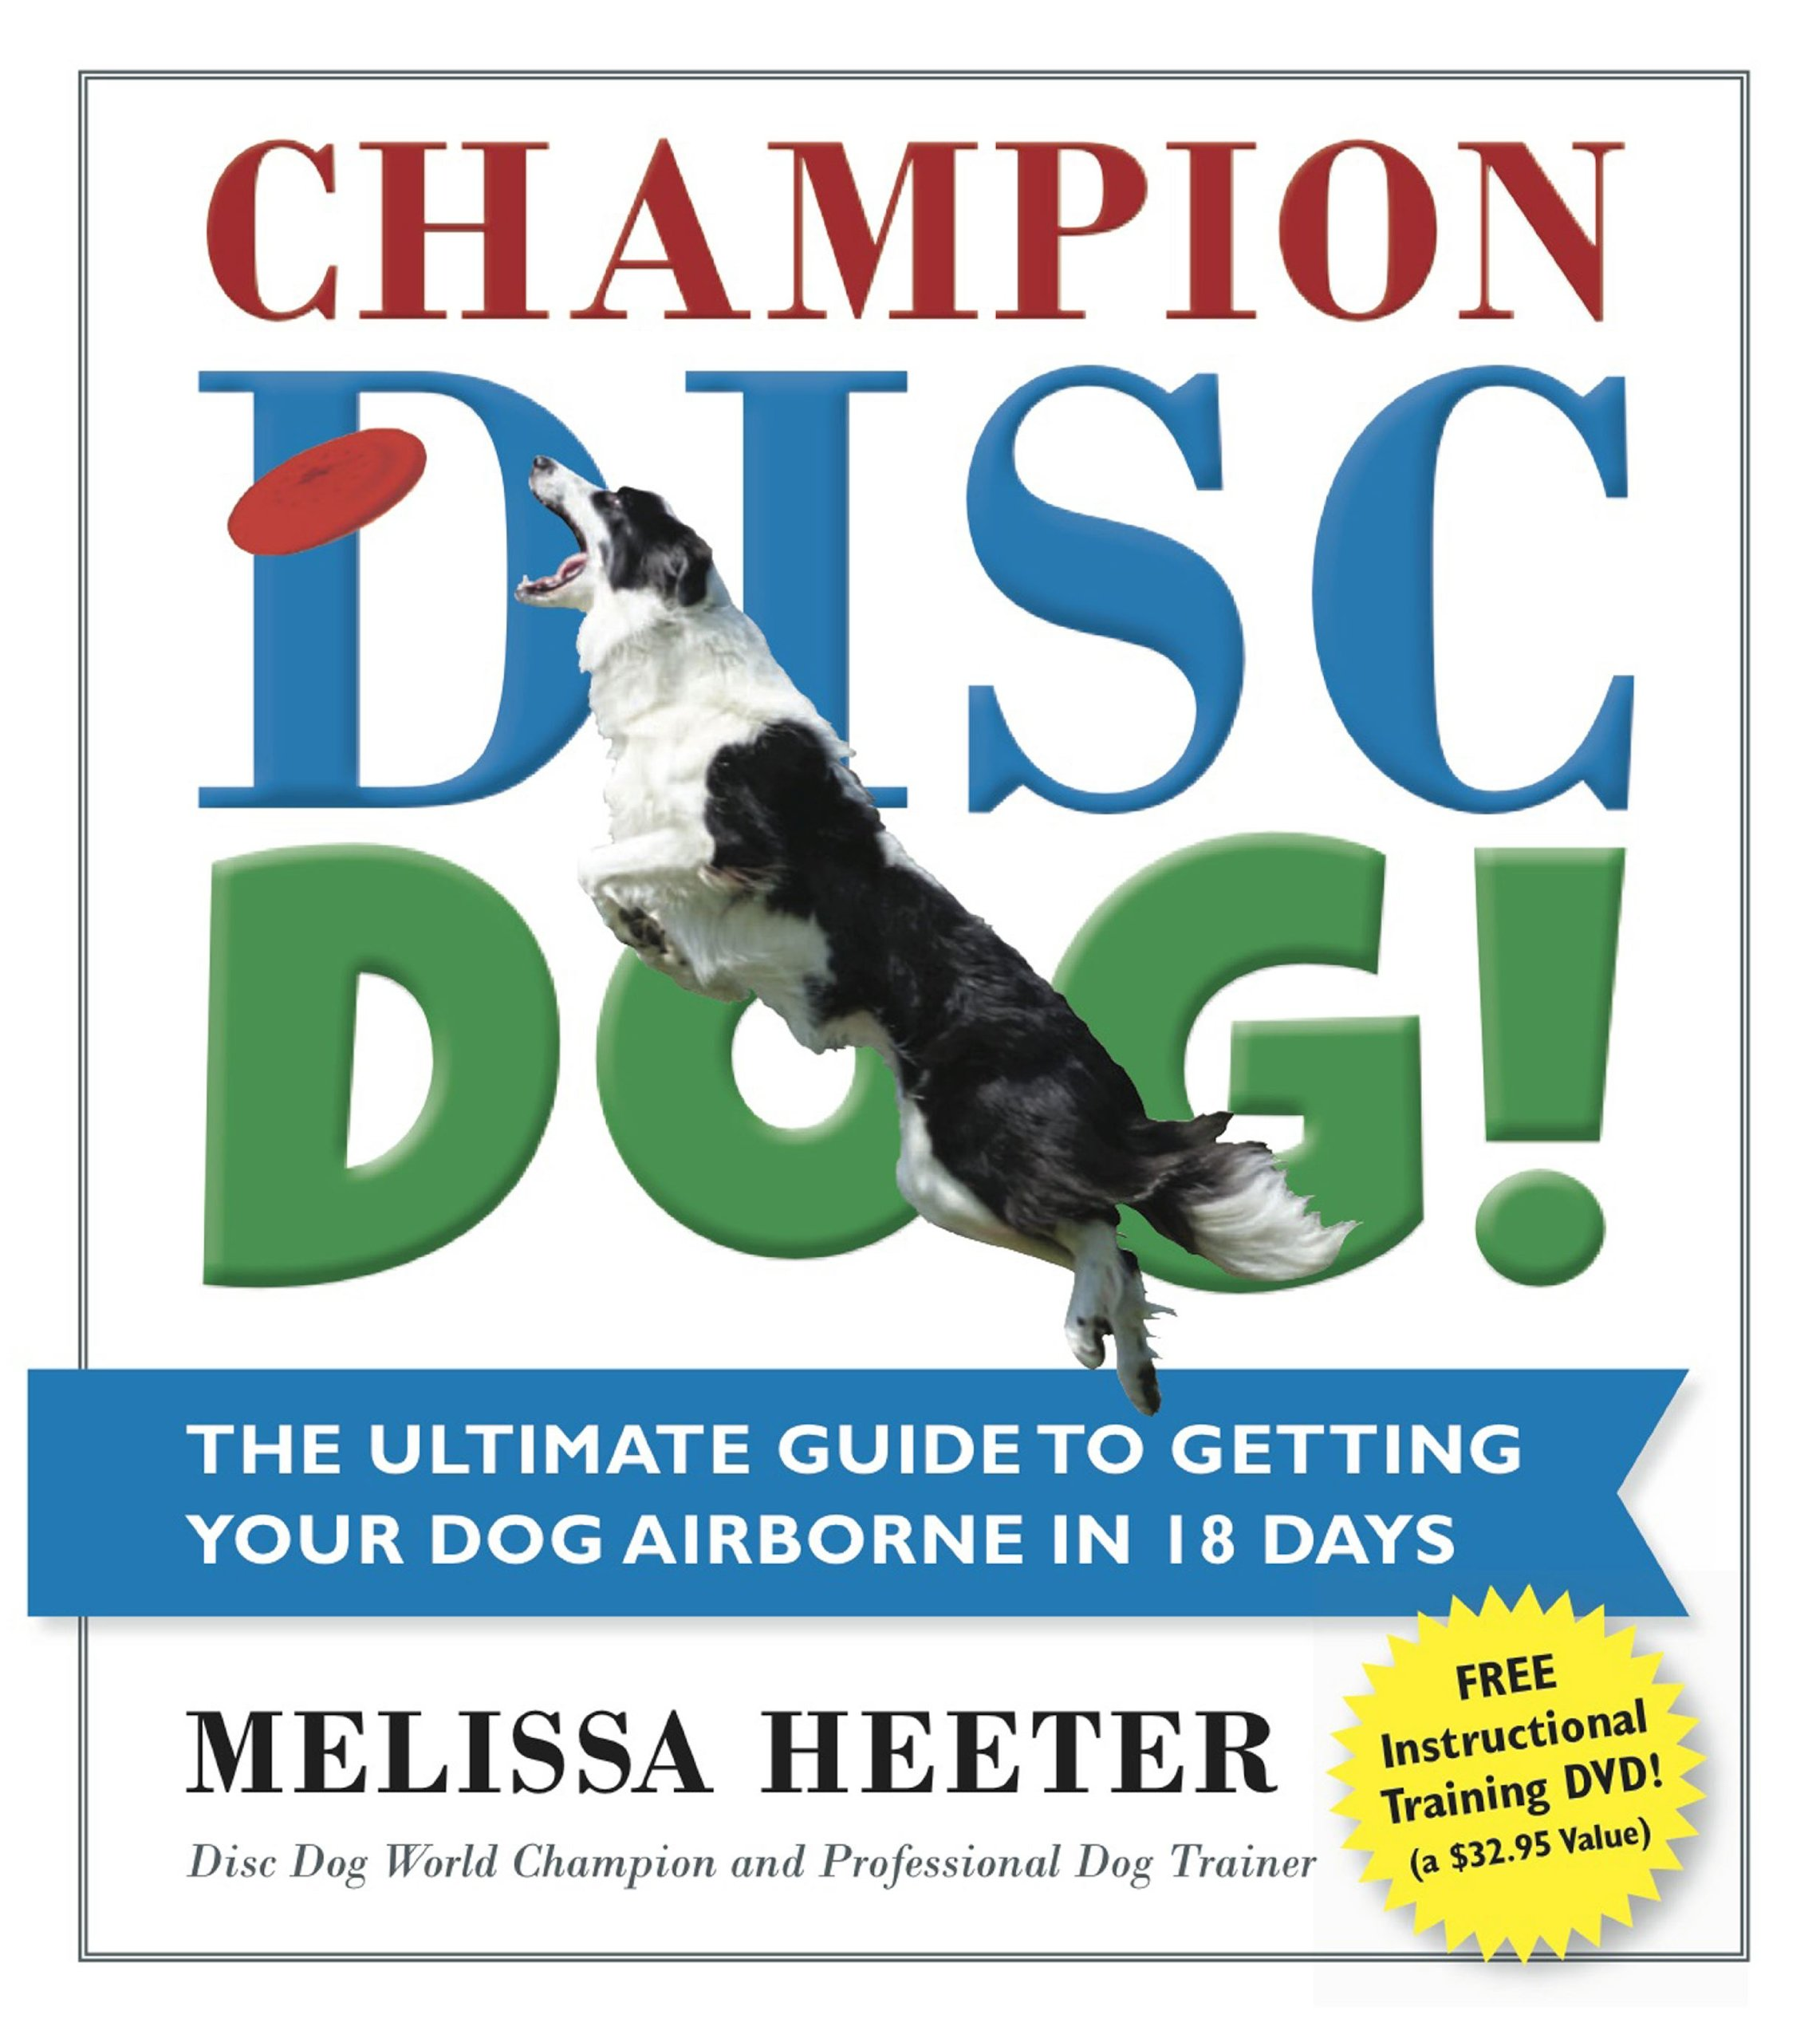
\includegraphics[height=.95\textheight]{static/discdog_book.jpg}
    \end{frame}

    \begin{frame}
        \centering
        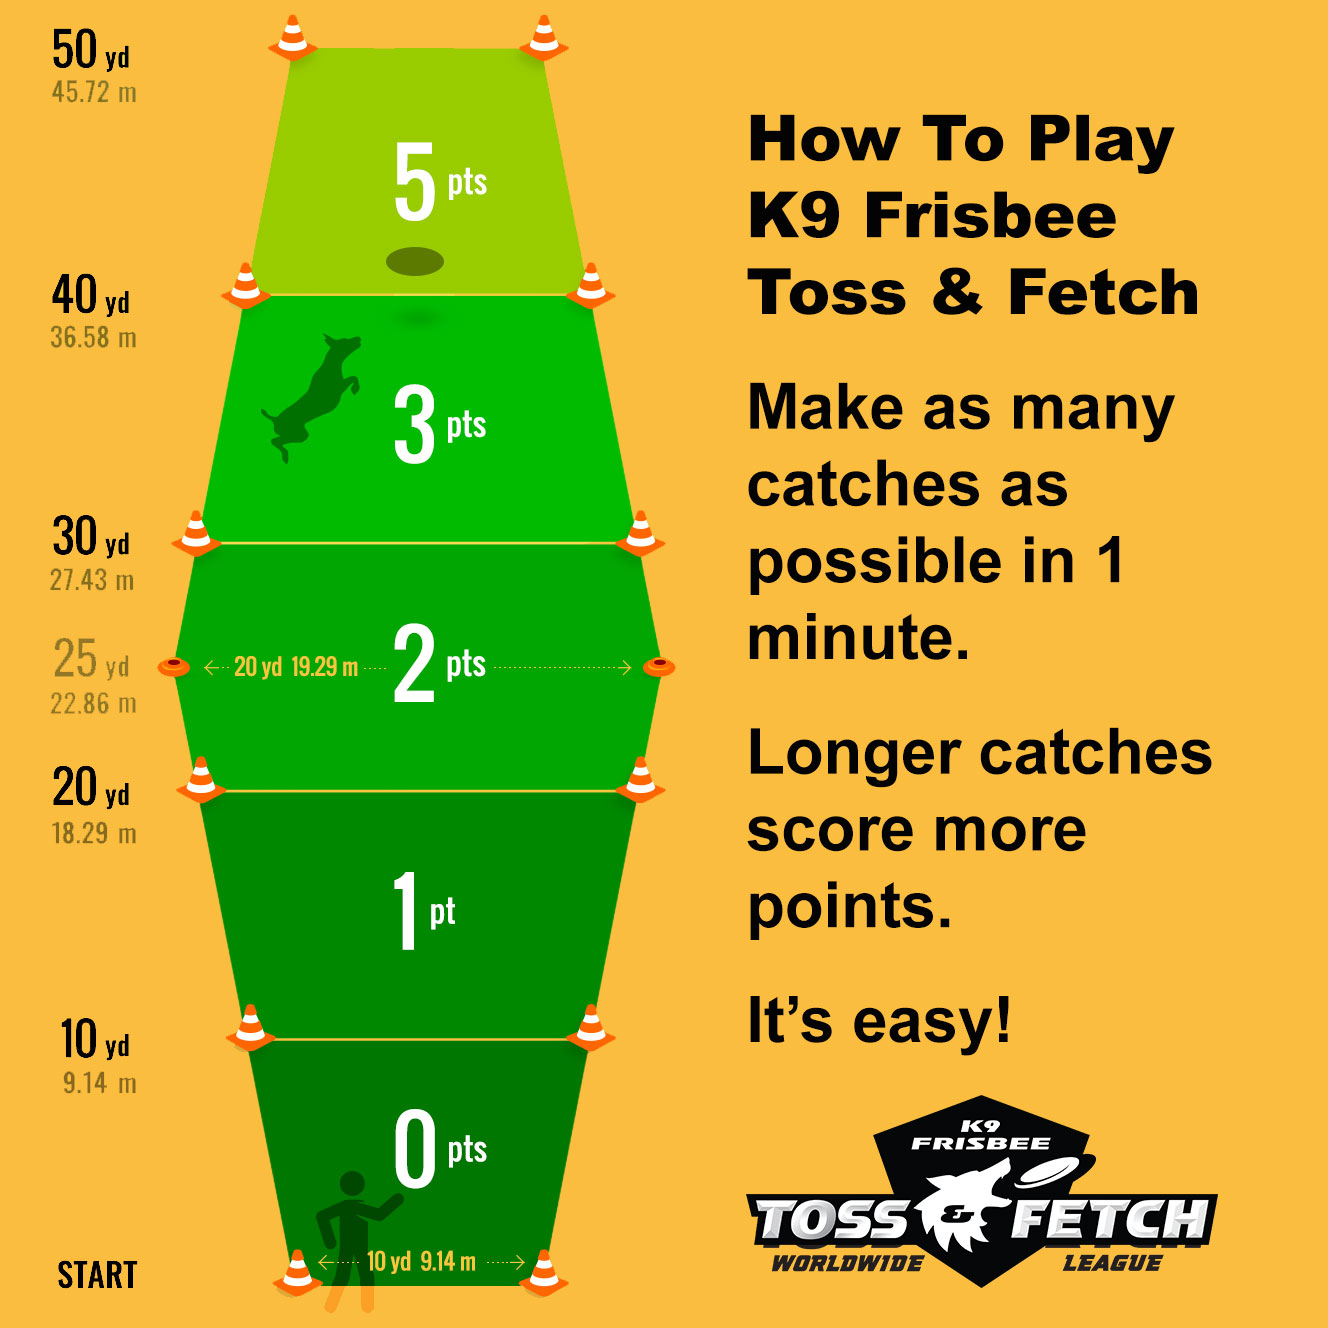
\includegraphics[height=.95\textheight]{static/toss_and_fetch.jpg}
    \end{frame}

    \begin{frame}
        \centering
        \Huge
        \framebox{
            \texttt{toss\_and\_fetch/}
    }
    \end{frame}

    \begin{frame}
        \centering
        \Huge
        Freestyle
    \end{frame}

    \begin{frame}
        \centering
        \Huge
        \framebox{
            \texttt{behaviours/}
    }
    \end{frame}

    \begin{frame}
        \centering
        \Huge
        \framebox{
            \texttt{sequences/}
    }
    \end{frame}

    \begin{frame}
        \centering
        \Huge
        Pup coach.
    \end{frame}

    \begin{frame}[fragile]
        \frametitle{\texttt{models.py}}
        \begin{minted}{python}
class Behaviour(models.Model):
    """A model for a behaviour"""
    created = models.DateTimeField(auto_now_add=True)
    title = models.CharField(
                max_length=100, 
                blank=True, 
                default=''
            )
    acquired = models.DateTimeField(auto_now_add=True)
    description = models.TextField(default='')

    class Meta:
        ordering = ('acquired',)

    def __str__(self):
        return self.title
        \end{minted}
    \end{frame}

    \begin{frame}[fragile]
        \frametitle{\texttt{urls.py}}
        \small
        \begin{minted}{python}
urlpatterns = [
    path('behaviours/', views.behaviour_list),
    path('behaviours/<int:pk>/', views.behaviour_detail),
    path(
        'behaviours/sequence/<int:length>/', 
        views.sequence_detail
        ),
    path(
        'behaviours/sequence/<int:length>/<int:seed>/', 
        views.sequence_detail
        ),
]

urlpatterns = format_suffix_patterns(urlpatterns)
        \end{minted}
    \end{frame}

    \begin{frame}[fragile]
        \frametitle{\texttt{views.py}}
        \small
        \begin{minted}{python}
@api_view(['GET', 'POST'])
def sequence_detail(request, length, seed=None, format=None):
    """
    Retrieve, update or delete a behaviour
    """
    if request.method == 'GET':
        if seed is not None:
            random.seed(seed)
        behaviours = random.sample(
                        list(Behaviour.objects.all()), 
                        length
                        )

        serializer = BehaviourSerializer(behaviours, many=True)
        return Response(serializer.data)
        \end{minted}
    \end{frame}

    \begin{frame}
        \centering
        \Huge
        \framebox{
            \texttt{routines/}
    }
    \end{frame}

    \begin{frame}
        \frametitle{Why DRF?}
        \begin{columns}
            \begin{column}{.5\textwidth}
                \begin{tikzpicture}
                    \node [draw] (db) at (0, 0) {Database};
                    \node [draw] (data) at ($(db) + (3, 0)$) {Data};
                    \node [draw] (html) at ($(data) + (0, -4)$) {Html};

                    \draw [->] (db) -- (data);
                    \draw [->] (data) -- (html);
                \end{tikzpicture}
            \end{column}
            \begin{column}{.5\textwidth}
                \centering
                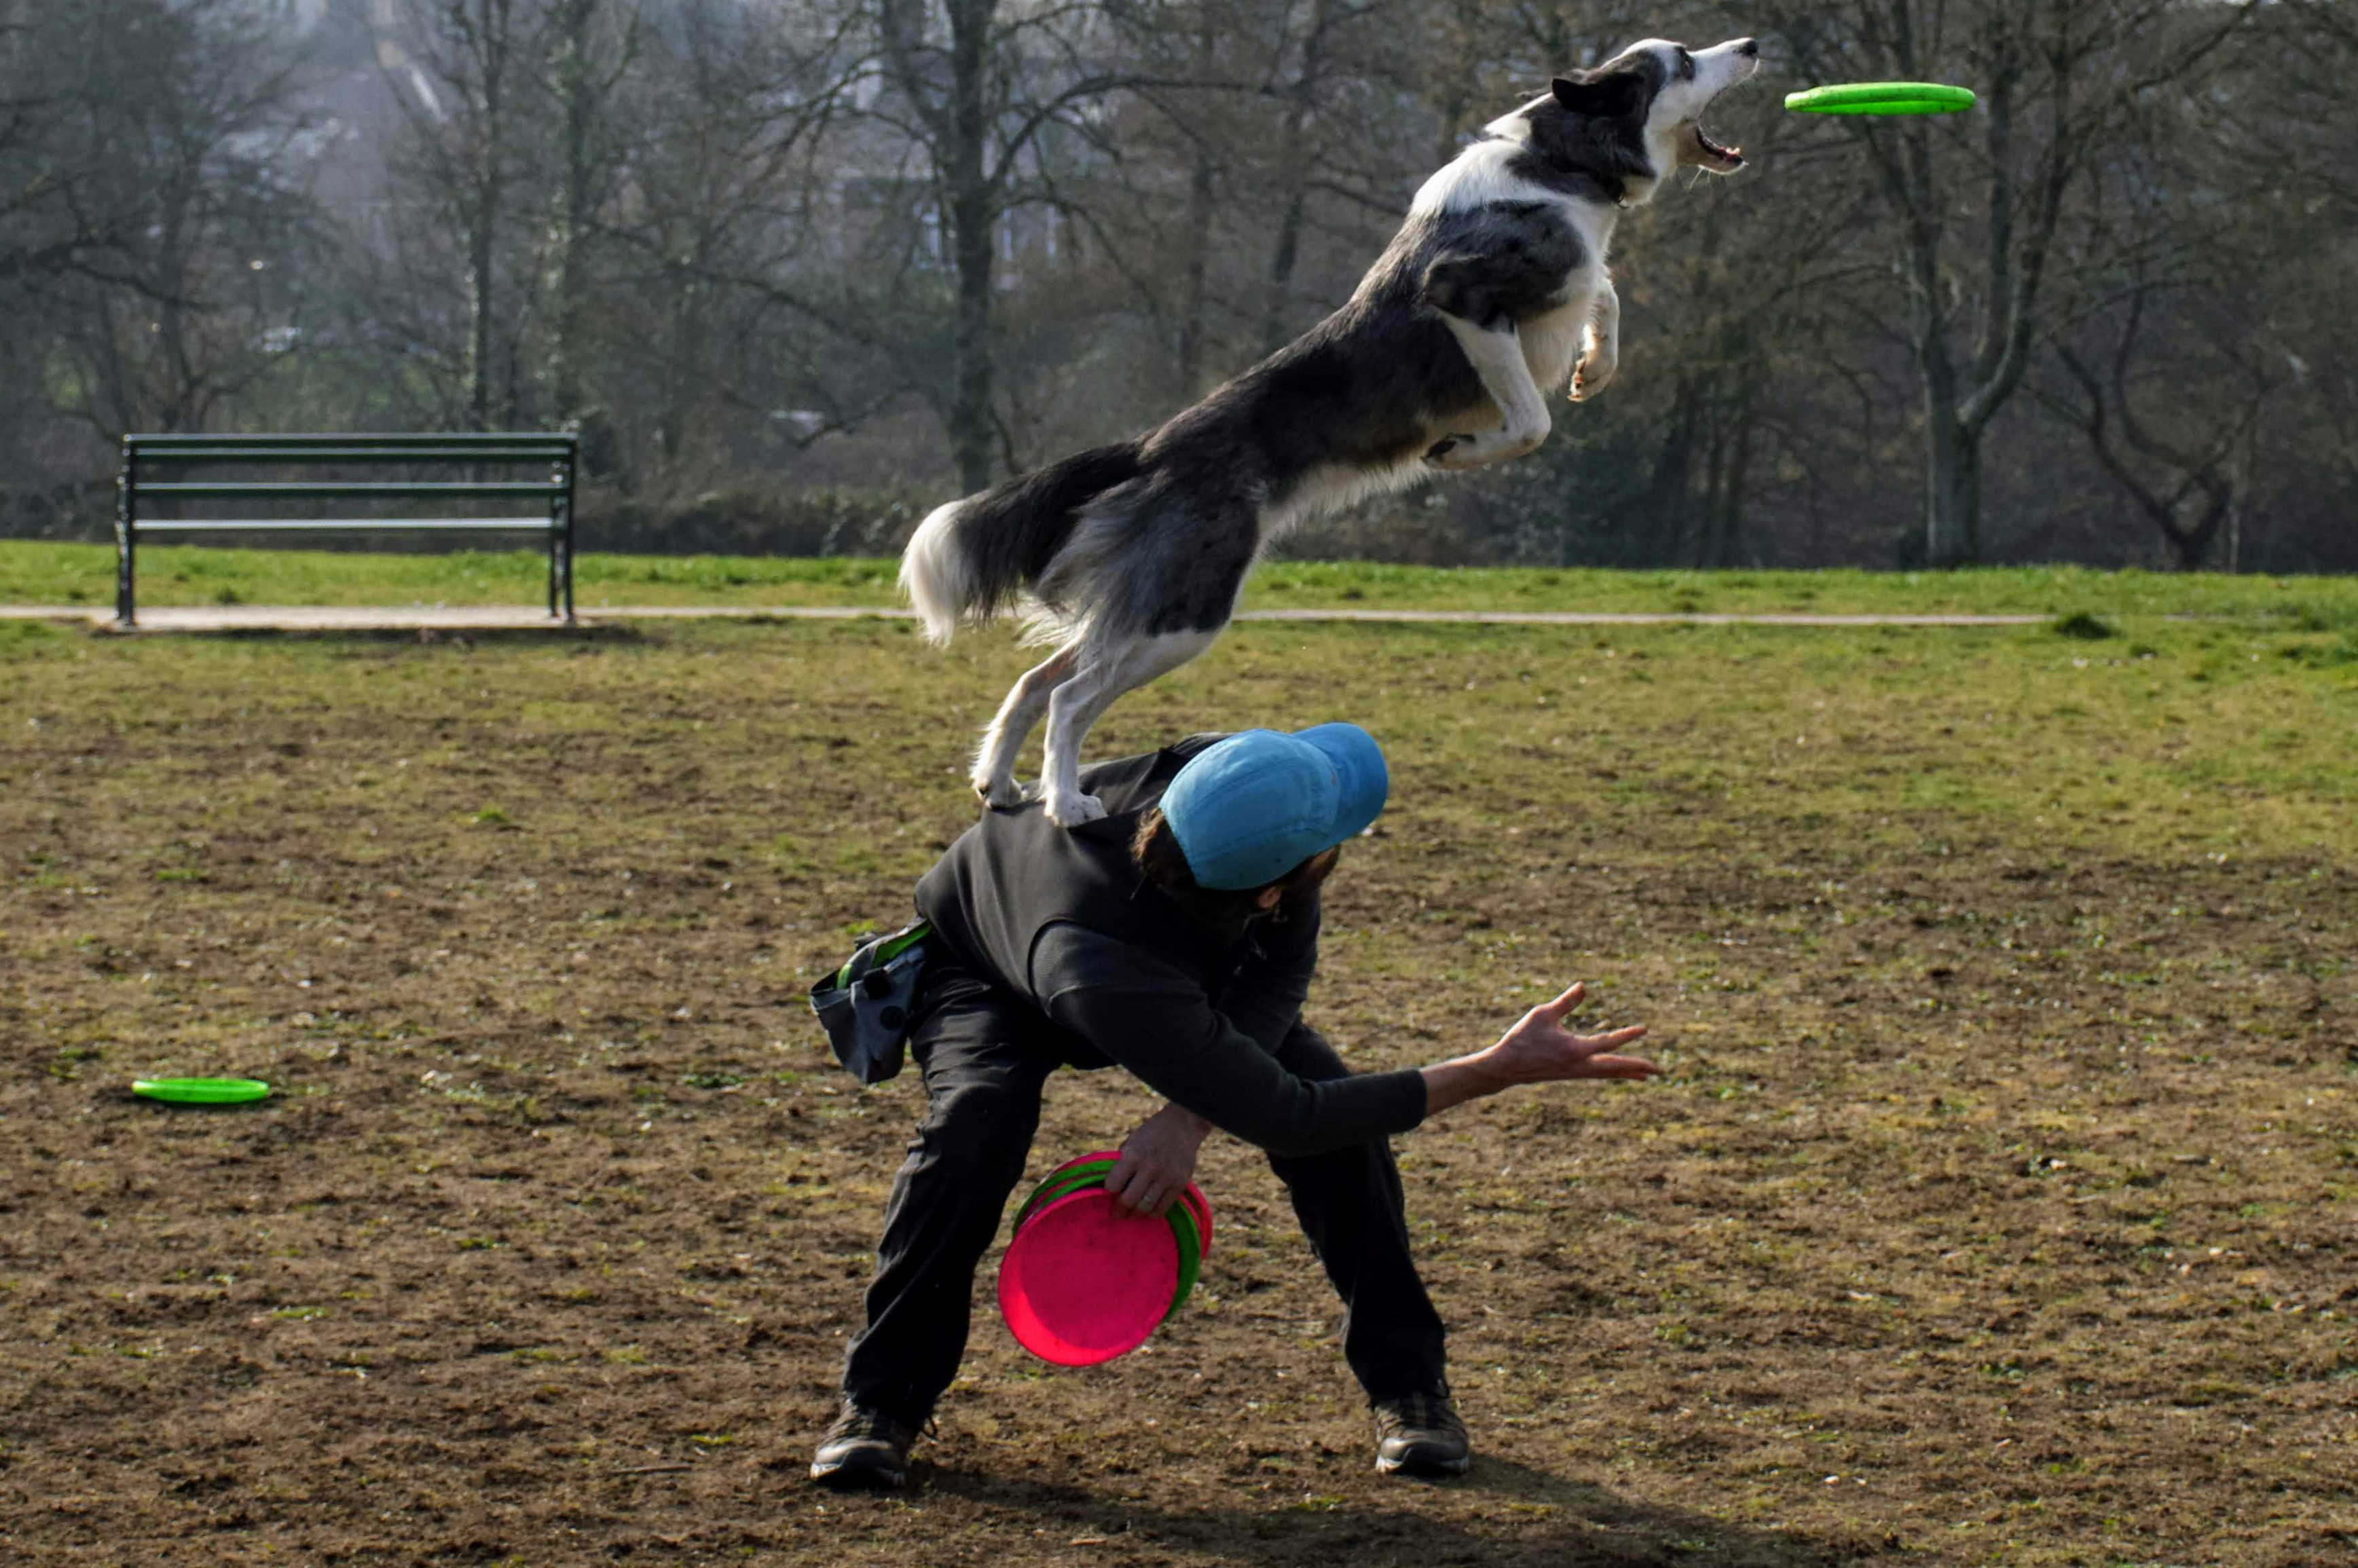
\includegraphics[width=\textwidth]{static/back_vault.jpg}
            \end{column}
        \end{columns}
    \end{frame}

    \begin{frame}
        \centering
        \Huge
        Reinforcement learning
    \end{frame}

    \begin{frame}
        \frametitle{Dog's health}
        \begin{columns}
            \begin{column}{.5\textwidth}
                \centering
                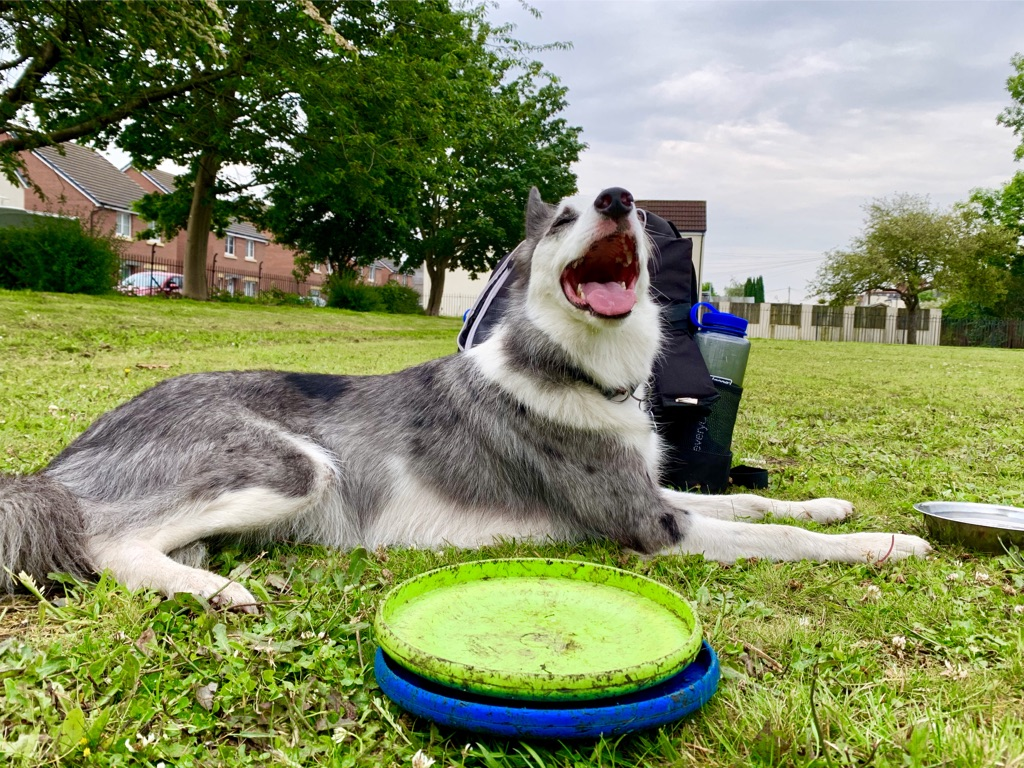
\includegraphics[width=\textwidth]{static/frisbees.jpg}
                \small
                \url{www.frisbeeschool.co.uk}
            \end{column}
            \begin{column}{.5\textwidth}
                \centering
                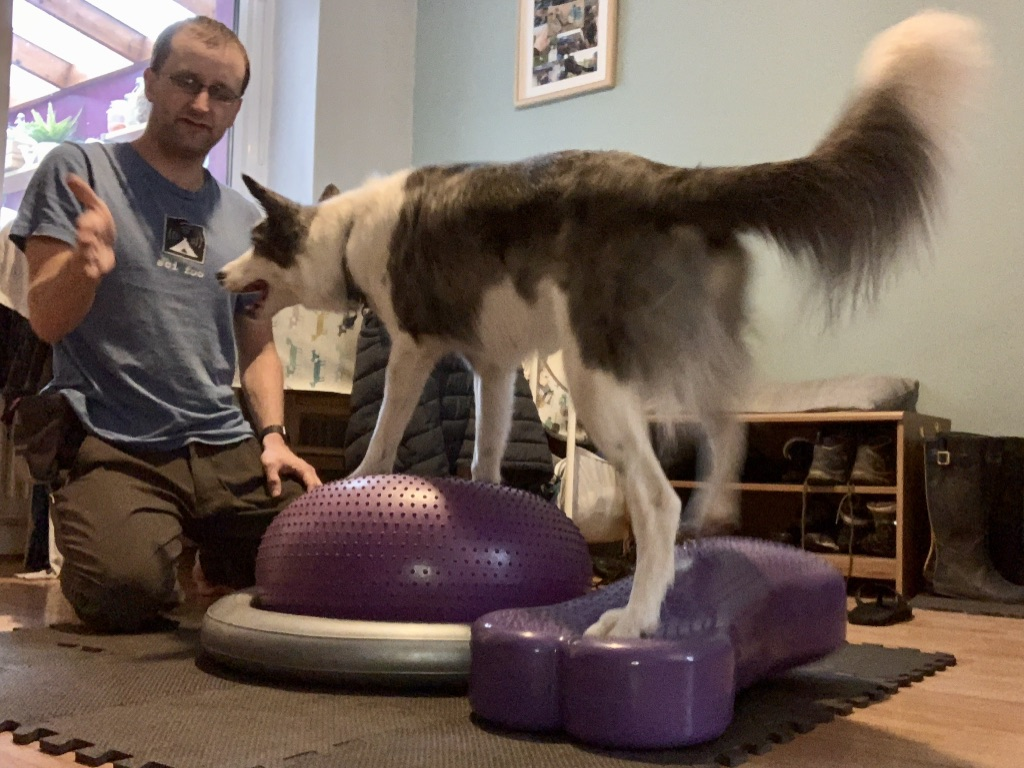
\includegraphics[width=\textwidth]{static/proprioception.jpg}
            \end{column}
        \end{columns}
    \end{frame}

    \begin{frame}
        \centering
        
        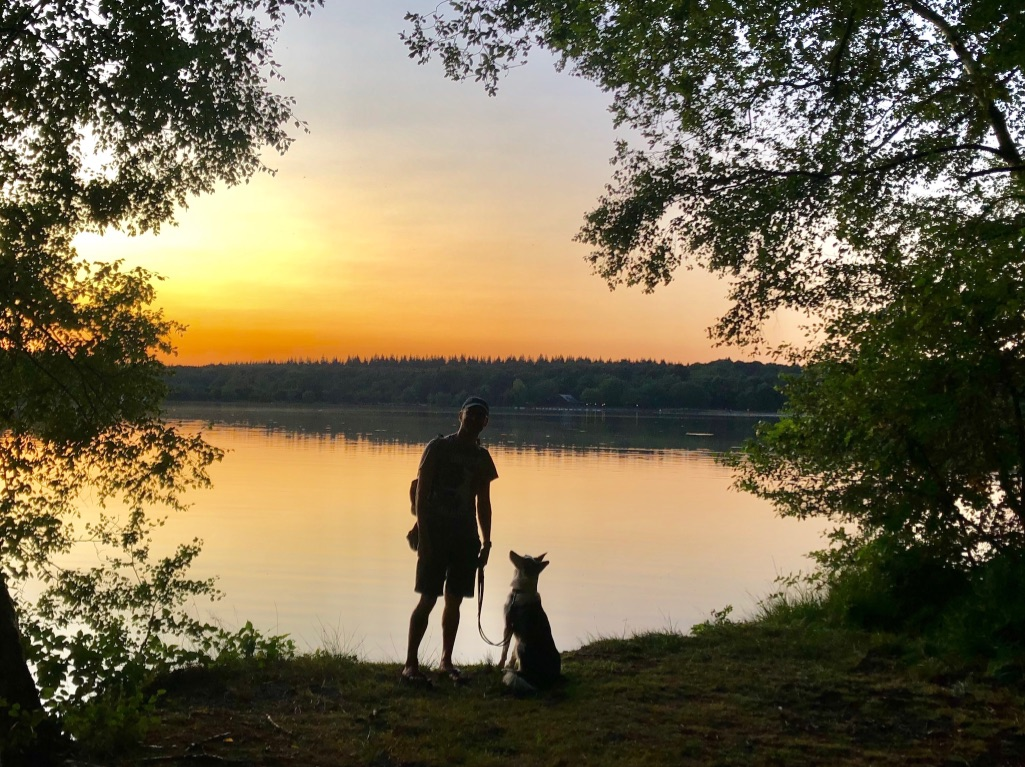
\includegraphics[width=.95\textwidth]{static/riggs_and_i_sunset.jpg}

    \end{frame}


    \begin{frame}
        \begin{columns}
            \begin{column}{.5\textwidth}
                \begin{itemize}
                    \item \url{@drvinceknight}
                    \item IG: \url{@vincent.prytherch}
                    \item Code: \url{github.com/drvinceknight/pupcoach}
                    \item Based on ``How to Build a Disc Dog Freestyle Routine
                    Step'' - Pawsitive vybe
                \end{itemize}
            \end{column}
            \begin{column}{.5\textwidth}
                \centering
                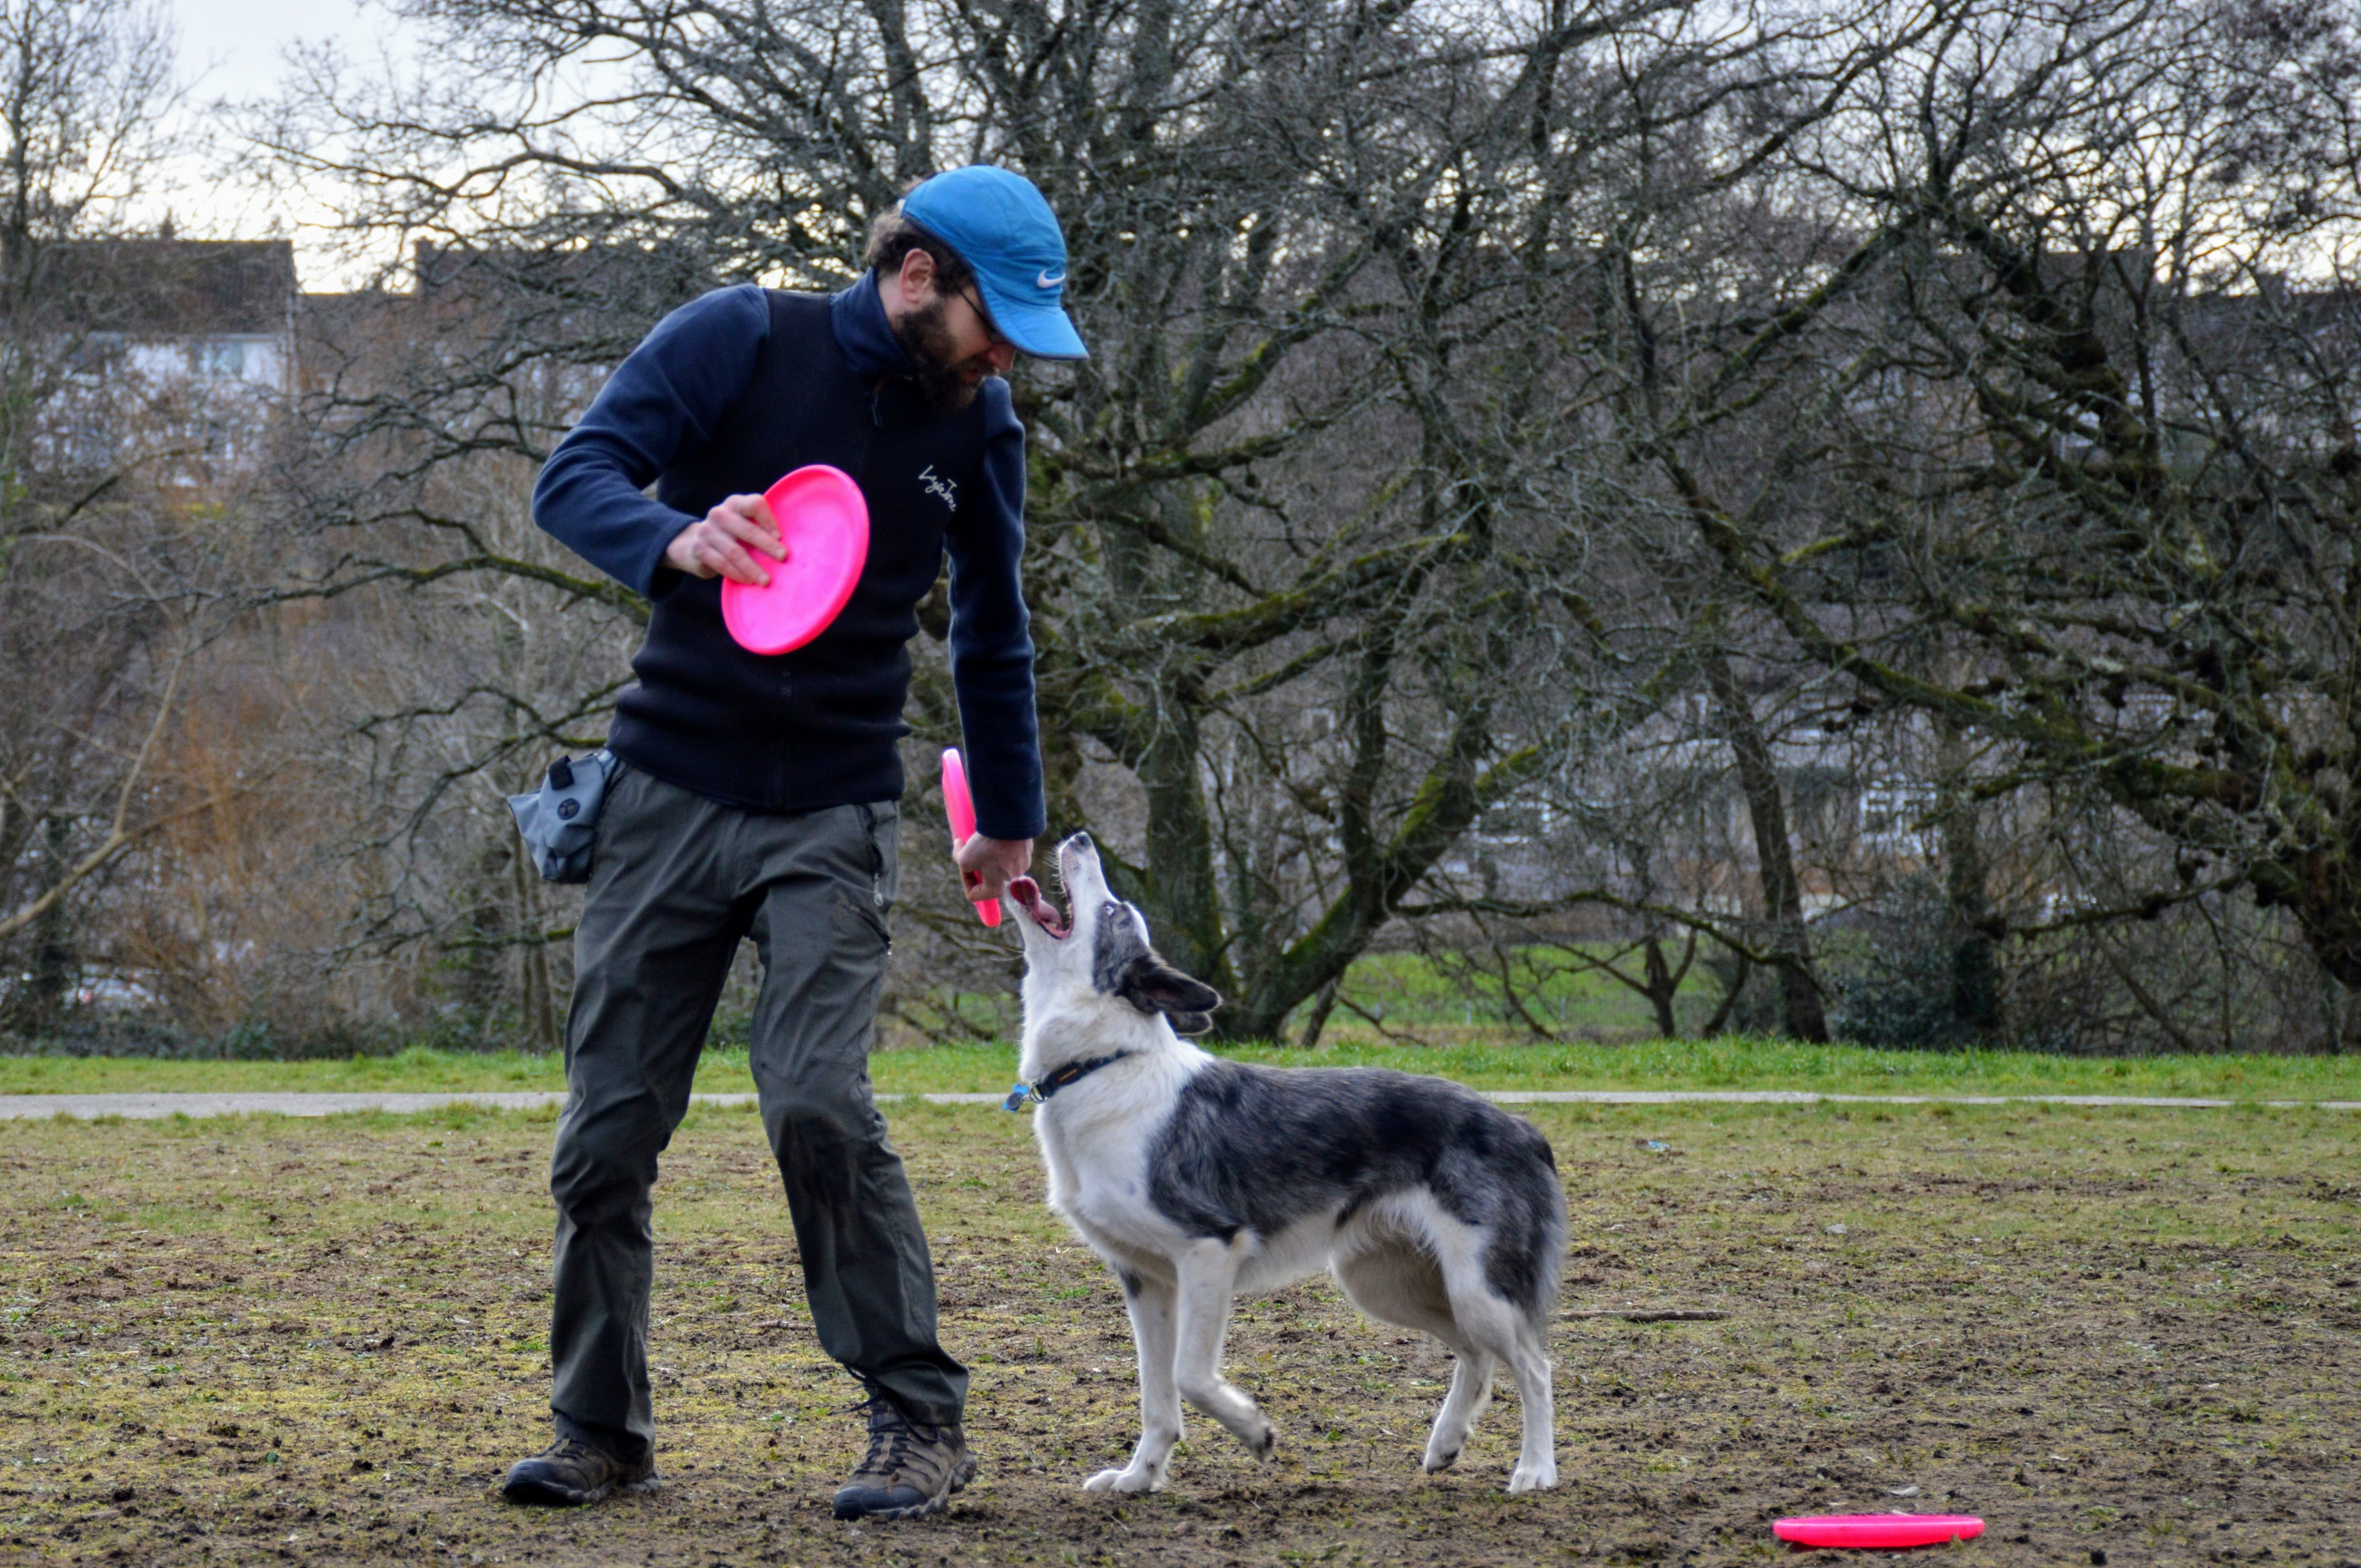
\includegraphics[width=\textwidth]{static/riggs_eyes_on_me.jpg}
            \end{column}
        \end{columns}
    \end{frame}

\end{document}
